% !TEX root = ../thesis.tex

\chapter{Evaluation}
\label{evaluation}

Dieses Kapitel dient der Evaluation der im vorangegangenen Kapitel erläuterten Klassifikationen. Dies geschieht durch verschiedene Evaluationsmetriken, welche in diesem Kapitel vorgestellt werden und auf Werten von sogenannten Konfusionsmatrizen basieren. Zudem umfasst dieses Kapitel eine Erläuterung von Herausforderungen und Limitationen, die im Laufe der Bearbeitung der Arbeit festgestellt worden sind. Abschließen wird dieses Kapitel ein Vergleich der Klassifikatoren zu einer klassischen dateibasierten Methode, welche aus der wissenschaftlichen Literatur entnommen wurde.
\\
\hrule

\section{Herausforderungen und Limitationen}

In diesem Abschnitt werden eine Reihe von Herausforderungen und Limitationen aufgezählt und erläutert, die im Rahmen der Erarbeitung auffällig wurden.

\subsection*{Identifikation von Features}

Die grundsätzliche Frage, die im Rahmen der Identifikation der Features aufkam, war: \glqq Was wird als Feature gezählt?\grqq. Wie bereits in \hyperref[construction]{Abschnitt 3.2} erwähnt wurde, barg die Identifikation der Features einige Herausforderungen. So gestaltete sich die erste Herausforderung in der Ausfilterung von \glqq Header-Features\grqq{}, die in einigen Programmierparadigmen verwendet werden, um Header-Dateien im Sourcecode einzubinden. Diese Header-Features erzeugen jedoch keine Variabilität im Code, sodass sie unerwünscht sind. Identifizierbar waren die meisten dieser Header-Features an ihren vergebenen Namen, welche ein \texttt{\_h\_} aufwiesen. Auf diesem Weg konnten sie mittels regulärer Ausdrücke schnell ermittelt und ausgefiltert werden. Es besteht jedoch auch die Möglichkeit, dass in einigen Softwareprojekten die Header-Features nicht explizit durch ihre Namensgebung kenntlich gemacht werden. Sie lassen sich somit nur schwer identifizieren, beispielsweise durch eine manuelle Sichtung der Kontexte der Features im Sourcecode. Dies wäre jedoch im vorliegenden Fall aufgrund der großen Menge an Features sehr zeitaufwändig und wurde aus diesem Grund nicht durchgeführt. Die Entfernung der erkennbaren Header-Features zeigte, dass ein erheblicher Teil der zuvor identifizierten Features unerwünscht war. Diese Methode erwies sich somit als effektiv.
Eine Lösung, die zu dem genannten Problem beitragen könnte, wäre ein Tool zum Parsen von Sourcecode zur korrekten Identifikation von Features mittels automatisierter Analyse des Kontextes des Features. So würden auch die erwähnten \glqq falschen\grqq{} Features ermittelt werden. Ein solches Tool existiert momentan jedoch nicht. Verfügbare Tools zur Identifikation von Features verwenden einen ähnlichen Ansatz, wie er in dieser Arbeit verwendet wurde (reguläre Ausdrücke).

\subsection*{Einbindung des Bezugs zu Features}
Wie in Kapitel 3 festgestellt werden konnte, basiert der Bezug zu den Features auf den ihnen zugrundeliegenden Dateien. Dazu wurden die Diffs der veränderten Dateien analysiert. Ein Feature gilt somit als relevant, wenn es in einem Diff Erwähnung findet. Es kann jedoch auch vorkommen, dass der enthaltene Featurecode nicht an der im Diff beschriebenen Veränderung beteiligt war. Es findet somit keine \glqq in-depth\grqq -Analyse des Sourcecodes statt. Dieser Weg wurde jedoch auch von der dieser Arbeit zugrundeliegenden wissenschaftlichen Arbeit gewählt \cite{Queiroz2016}. Ebenfalls werden die Metriken der Features auf Basis der Metadaten der zugrundeliegenden Dateien berechnet.

\subsection*{Heuristik zur Erkennung von korrektiven Commits}

Die Heuristik zur Erkennung von korrektiven Commits wurde im Verlauf der Erarbeitung der Arbeit geändert. Zunächst wurde die gesamte Commit-Nachricht auf das Vorhandensein der Schlagworte analysiert. Dies führte jedoch dazu, dass einige Commits fälschlicherweise als korrektiv identifiziert wurden. Der Grund dafür war, dass die Commit-Nachrichten in einigen der verwendeten Softwareprojekte sehr umfangreich in der Anzahl der Wörter waren. In diesen Nachrichten wurden ausnahmslos alle Veränderungen, die mit den Commits vorgenommen wurden, erwähnt. Dabei handelte es sich jedoch meist um für diesen Zweck irrelevante Veränderungen. Es wurde festgestellt, dass sich die Hauptaussage beziehungsweise der Hauptgrund des Commits in der ersten Zeile der Commit-Nachricht befindet. Die Heuristik wurde daraufhin dementsprechend angepasst. Eine Stichprobe von korrektiven Commits vor und nach der Anpassung der Heuristik zeigte, dass die Veränderung dazu führte, dass tatsächlich irrelevante korrektive Commits entfernt wurden.

\subsection*{Unpräzisiertheit des SZZ-Algorithmus}

Eine Limitation, die im Laufe der Erstellung des Datensets durch Literaturrecherchen festgestellt wurde, bezieht sich auf den SZZ-Algorithmus. Dieser wurde genutzt, um fehlereinführende Commits auf Basis der Commit-Hashes der korrektiven Commits zu identifizieren. Analysen des Algorithmus ergaben, dass momentan verfügbare Implementationen und somit auch die des verwendeten Python-Tools PyDriller lediglich etwa 69\% der tatsächlich existierenden fehlereinführenden Commits identifizieren können \cite{Wen2019}. Darüber hinaus wurde herausgefunden, dass etwa 64\% der identifizierten Commits falsch ermittelt wurden \cite{Wen2019}. Der Algorithmus gilt somit als unpräzise \cite{Wen2019}. Die Begründung dafür lautet wie folgt:

\begin{quotation}
The reason is that the implicit assumptions of the SZZ algorithm
are violated by the insufficient file coverage and statement direct
coverage between bug-inducing and bug-fixing commits. - \cite{Wen2019}
\medskip \\
\textit{Der Grund dafür ist, dass die impliziten Annahmen des SZZ-Algorithmus durch die unzureichende \glqq file coverage\grqq{} und die unzureichende \glqq statement direct
coverage\grqq{} der Aussage zwischen fehlereinführenden und korrektiven Commits verletzt werden.}
\end{quotation}

Ferner stellten die Autoren der Studie in eigenen durchgeführten Tests fest, dass die Ergebnisse von acht von zehn früheren Studien durch den unpräzisen Algorithmus signifikant beeinflusst wurden \cite{Wen2019}. Dies kann somit auch auf diese Arbeit zutreffen. Es existiert jedoch momentan keine alternative Methode zur Identifizierung von fehlereinführenden Commits. Sollte eine neue Methode oder eine verbesserte Version des SZZ-Algorithmus veröffentlicht werden, so würde es sich anbieten, die Hauptschritte dieser Arbeit unter Berücksichtigung der neuen Methode zu wiederholen, um sie mit den hier vorliegenden Ergebnissen zu vergleichen, um die Einflüsse des SZZ-Algorithmus herauszustellen.

\subsection*{Vorhersageziel}
commits, releases?
\textbf{absprechen mit Daniel ...}

\section{Vergleich der Klassifikatoren}

Der Vergleich der Klassifikatoren erfolgt unter Zuhilfenahme von Evaluationsmetriken, die im nachfolgenden Abschnitt vorgestellt werden. Die Diskussion der Ergebnisse der Evaluation erfolgt in \hyperref[results]{Abschnitt 5.2.2}.

\subsection{Evaluationsmetriken}
\label{eval-metrics}

Die zum Vergleich der Klassifikatoren erhobenen Evaluationmetriken entstammen dem Themengebiet des Information Retrieval und gelten als Standardmesswerte für ihren Einsatzzweck \cite{Sammut2017}. Die meisten dieser Metriken lassen sich anhand von Werten einer sogenannten Konfusionsmatrix berechnen und messen allesamt die Performanz der Vorhersagen von Klassifikatoren unter verschiedenen Betrachtungsweisen. Im Falle einer binären Klassifikation, wie in dieser Arbeit, besteht diese Matrix aus vier Gruppen, deren Werte angeben, ob der jeweilige Klassifikator ein Objekt korrekt oder falsch einer der beiden Zielklassen zuordnen konnte \cite{Sammut2017}. Im Zusammenhang mit solchen Matrizen werden die beiden Zielklassen \glqq positiv\grqq{} und \glqq negativ\grqq{} genannt. Für diese Arbeit werden die positive Klasse dem Label \glqq fehlerfrei\grqq und die negative Klasse dem Label \glqq defekt\grqq{} zugeordnet. Die Form einer allgemeinen Konfusionsmatrix ist in \autoref{fig:confu} dargestellt.

\begin{figure}[H]
    \centering
    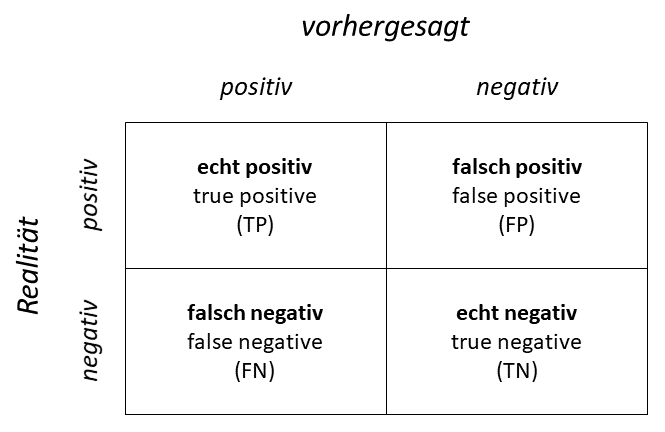
\includegraphics[width=0.7\textwidth]{images/Confusion}
    \caption{allgemeine Konfusionsmatrix\label{fig:confu}}
\end{figure}

Sowohl scitkit-learn als auch WEKA besitzen die Option, Konfisionsmatrizen zu den durchgeführten Tests der Klassifikatoren auszugeben. Anhand der Werte der Zuordnungen zu den zuvor genannten Gruppen wurden die folgenden Evaluationsmetriken berechnet: 

\begin{itemize}
\item Treffergenauigkeit (Accuracy)
\\Dieser Wert misst die Treffergenauigkeit der Vorhersagen des Klassifikators und gibt an, inwieweit dessen Vorhersagen mit der modellierten Realität übereinstimmen \cite{Sammut2017}. Die Formel zur Berechnung der Accuracy lautet:
\\\[Accuracy = \frac{TP+TN}{TP+TN+FP+FN}\]
Das Ergebnis der Berechnung ist ein prozentualer Wert. 100\% stellen damit die bestmögliche Accuracy dar.
\item Echt-Positiv-Rate / Trefferquote (TP-Rate / Recall)
\\Dieser Wert gibt den Anteil der korrekt als positiv gewerteten Vorhersagen sämtlicher als positiv gewerteter Vorhersagen an \cite{Alpaydin2010}. Die Formel zur Berechnung der TP-Rate bzw. des Recalls lautet:
\\\[TP-Rate = \frac{TP}{TP+FN}\]
Das Ergebnis der Berechnung ist ein prozentualer Wert. 100\% stellen damit die bestmögliche TP-Rate bzw. den bestmöglichen Recall dar. Beide Begriffe werden parallel für die Berechnung der gezeigten Formel verwendet.
\item Positiver Vorhersagewert (Precision)
\\ Dieser Wert gibt die Anzahl der positiven Vorhersagen an, die auch tatsächlich zur positiven Klasse gehören \cite{Sammut2017}. Die Formel zur Bestimmung der Precision lautet:
\\\[Precision = \frac{TP}{TP+FP}\]
Das Ergebnis der Berechnung ist ein prozentualer Wert. 100\% stellen damit die bestmögliche Precision dar.
\item F-Maß (F-Score)
\\ Dieser Wert berechnet das harmonische Mittel der Werte Precision und Recall und liegt somit zwischen diesen beiden Werten, jedoch näher am kleineren Wert \cite{Sammut2017}. Die Formel zur Berechnung des F-Scores lautet:
\\\[F-Score = \frac{2TP}{2TP+FP+FN}\]
Das Ergebnis der Berechnung ist ein prozentualer Wert. 100\% stellen damit den bestmöglichen F-Score dar.
\end{itemize}

\label{roc-def}
Darüber hinaus wurden die sogenannten ROC-Kurven (ROC curve) der einzelnen Klassifikatoren ermittelt. Diese Wahrscheinlichkeitskurven bzw. -graphen (ROC = Receiver Operating characteristic, Betriebsverhalten des Empfängers), beschreiben das Verhältnis zwischen der TP-Rate (y-Achse) und der FP-Rate (x-Achse) \cite{Sammut2017,Narkhede2018}. Die Falsch-Positiv-Rate (FP-Rate) gibt dabei den Anteil der fälschlicherweise als positiv gewerteten Vorhersagen an \cite{Alpaydin2010}. Sie wird mittels der folgenden Formel berechnet:
\\\[FP-Rate = \frac{FP}{FP+TN}\]

Wie bei allen Metriken ist das Ergebnis der FP-Rate ein prozentualer Wert, der bestenfalls möglichst gering ausfallen sollte. Sowohl die TP-Rate als auch die FP-Rate geben nur singuläre Werte an, aus welchen sich keine Graphen herleiten lassen. Jeder Klassifikator errechnet jedoch im Rahmen der Vorhersage eines Datensatzes Wahrscheinlichkeiten, die die Zugehörigkeit zu den Werten der Zielklasse darstellen \cite{KNIMETV2019}. In der Regel wird ein Datenpunkt der positiven Klasse zugeordnet, wenn die Wahrscheinlichkeit einen Schwellenwert von 0,5 übersteigt - Datenpunkte, die diesen Schwellenwert unterschreiten werden wiederum der negativen Klasse zugeordnet \cite{KNIMETV2019}. Wird der Schwellenwert erhöht, so werden weniger Datenpunkte der positiven Klasse zugeordnet, wohingegen im Falle einer Absenkung des Schwellenwertes mehr Datenpunkte der positiven Klasse zugeordnet werden \cite{KNIMETV2019}. Für die Erstellung der ROC-Kurven werden somit die Werte der TP-Rate und der FP-Rate unter der Berücksichtigung der Schwellenwerte im Bereich von 0,0 bis 1,0 gegenübergestellt.

Eine weitere Metrik, die in Verbindung mit der ROC-Kurve auftritt, ist der ROC-Bereich (ROC area). Dieser Wert, der anhand der ROC-Kurve berechnet wird und auch AUC-Bereich (AUC = Area Under Curve, Bereich unter der Kurve) genannt wird, gibt an, in wieweit ein Klassifikator in der Lage ist, zwischen den Werten der Zielklassen zu unterscheiden \cite{Narkhede2018}. Je höher dieser Wert ist (1,0 ist das Maximum), desto besser trifft der Klassifikator korrekte Vorhersagen \cite{Narkhede2018}.

Am Beispiel des Schwellenwertes 0,5 wird nun die Interpretation der ROC-Kurve und des ROC-Bereiches vorgenommen. Unterstützt wird dies durch grafische Beispiele, die in \autoref{fig:curves} gezeigt werden. Der Idealfall ist in den (a) und (b) dargestellt. Die Wahrscheinlichkeitskurven der Zielklasse (a) weisen keine Überlappung auf. Die Werte der Zielklasse sind somit allesamt korrekt zugeordnet worden, sodass der Klassifikator korrekt zwischen diesen unterscheiden kann. Die diesem Fall entsprechende ROC-Kurve ist in (b) dargestellt. Der ROC-Bereich beträt in diesem Fall 1,0. Ein \glqq Normalfall\grqq{} ist in (c) und (d) dargestellt. Es ist in (c) zu erkennen, dass die Wahrscheinlichkeitskurven überlappen, sodass falsche Zuordnungen getroffen werden. Die entsprechende ROC-Kurve ist in (d) dargestellt. Der entsprechende ROC-Bereich beträgt im hier gezeigten Fall 0,7. Dies bedeutet, dass 70\% der Zuordnungen richtig getroffen werden. Verbessert werden können die Werte möglicherweise, wenn der Schwellenwert verändert wird. Der \glqq Worst Case\grqq, der bei der Performanzmessung mittels ROC-Kurven auftreten kann, ist in (e) und (f) dargestellt. In (e) ist zu erkennen, dass sich die Wahrscheinlichkeitskurven vollständig überlappen. Es findet somit eine willkürliche Zuordnung statt. Die zugehörige ROC-Kruve (f) entspricht einer Winkelhalbierenden. Ein weiterer Fehlerfall ist in (g) und (h) dargestellt. Die Wahrscheinlichkeitskurven (g) zeigen, dass die Zuordnungen gegenteilig erfolgen und somit der jeweils dem anderen Wert der Zielklasse falsch zugeordnet werden. Der entsprechende ROC-Bereich beträgt 0, da wie in (h) zu sehen ist, keine Fläche unter der Kurve vorhanden ist.

\begin{figure}[t]
  \centering
  \subfloat[][Idealfall]{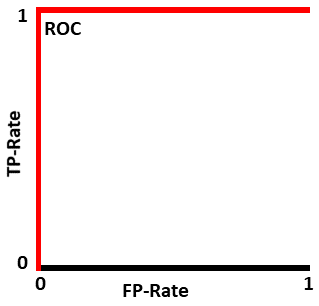
\includegraphics[width=0.5\linewidth]{images/roc_ideal}}
  \subfloat[][Idealfall]{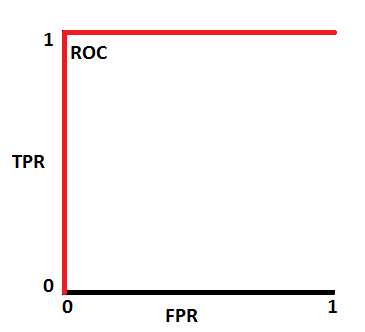
\includegraphics[width=0.25\linewidth]{images/roc_ideal_curve}}
  \qquad
  \subfloat[][\glqq Normalfall\grqq]{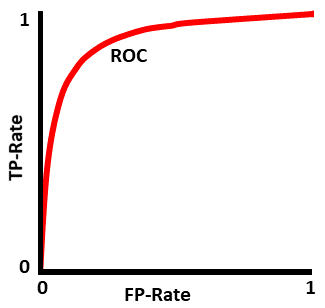
\includegraphics[width=0.5\linewidth]{images/roc_normal}}
  \subfloat[][\glqq Normalfall\grqq]{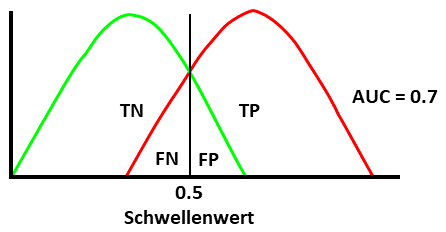
\includegraphics[width=0.25\linewidth]{images/roc_normal_curve}}
  \qquad
  \subfloat[][\glqq Worst Case\grqq]{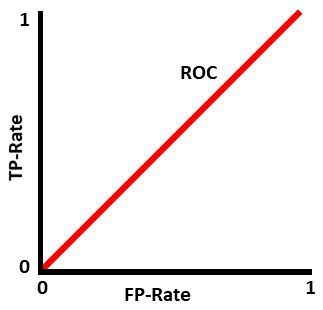
\includegraphics[width=0.5\linewidth]{images/roc_worst}}
  \subfloat[][\glqq Worst Case\grqq]{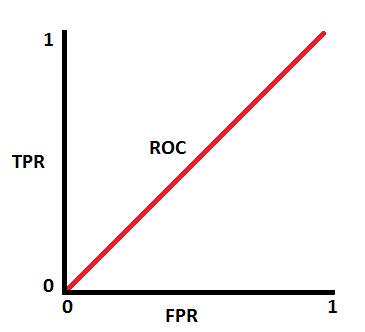
\includegraphics[width=0.25\linewidth]{images/roc_worst_curve}}
  \qquad
  \subfloat[][Fehlerfall]{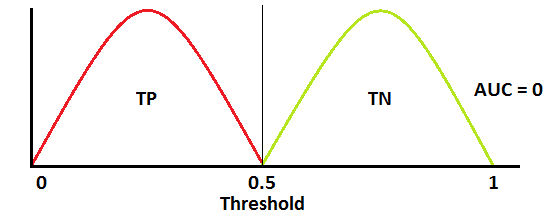
\includegraphics[width=0.5\linewidth]{images/roc_neg}}
  \subfloat[][Fehlerfall]{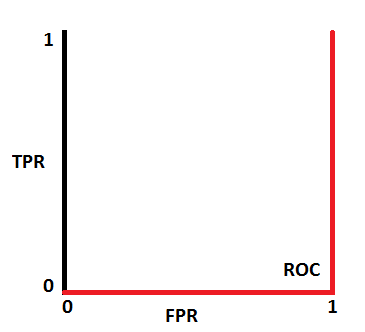
\includegraphics[width=0.25\linewidth]{images/roc_neg_curve}}
  \caption{Beispiel zur Interpretation der ROC-Kurve und des ROC-Bereiches (TPR = TP-Rate, FPR = FP-Rate, Threshold = Schwellenwert) \cite{Narkhede2018}
\label{fig:curves}}
\end{figure}

Alle vorgestellten Metriken werden automatisiert von den Werkzeugen scikit-learn und WEKA berechnet. Ferner besitzen beide Werkzeuge die Fähigkeit, ROC-Kurven mit den entsprechenden ROC-Werten auszugeben. Die im Rahmen der Evaluation der Klassifikatoren ermittelten Werte der Metriken sowie die ROC-Kurven und Werte der ROC-Bereiche werden im folgenden Abschnitt aufgeführt sowie innerhalb sowie zwischen den Datensets verglichen und interpretiert.

\fbox{\parbox{\linewidth}{RQ3a: WELCHE MITEINANDER VERGLEICHBAREN MERKMALE BESITZEN DIE KLASSIFIKATOREN?\medskip\\
Die Merkmale zum Vergleich stellen Evaluationsmetriken dar, welche auf Basis der Ergebnisse des Tests der Klassifikatoren errechnet werden und die Performanz der Vorhersagen auf verschiedene Weisen messen. Welche Metriken berechnet wurden beantwortet Forschungsfrage RQ3b.}}

\fbox{\parbox{\linewidth}{RQ3b: WELCHE METRIKEN KÖNNEN FÜR DEN VERGLEICH VERWENDET WERDEN?\medskip\\
Für den Vergleich der Klassifikatoren werden klassische Evaluationsmetriken verwendet, welche auf Basis von Konfusionsmatrizen berechnet werden. Die betrachteten Metriken lauten: Accuracy, TP-Rate, Precision und F-Score. Ebenfalls hinzugezogen werden die jeweiligen ROC-Kurven der Klassifikatoren inklusive der ROC-Bereiche. Diese Metriken stellen einen Standard für die Messung der Performanz der Vorhersagen von Klassifikatoren dar.}}

\subsection{Ergebnisse und Diskussion}
\label{results}

\subsubsection*{Konfusionsmatrizen}

Als Basis der Ergebnisse der Evaluation der Klassifikatoren anhand der zuvor vorgestellten Metriken dienen die Konfusionsmatrizen. Die Matrizen des featurebasierten Datensets sind in \autoref{tab:mat-feat} aufgeführt, die Matrizen des dateibasierten Datensets können in \autoref{tab:mat-file} gefunden werden. Beide Tabellen sind in den Spalten in die beiden verwendeten Tools scikit-learn und WEKA unterteilt. Ferner bilden die Spalten die von den Klassifikatoren vorhergesagten Label ab, wohingegen die Zeilen die \glqq ground truth\grqq, also die Realität, abbilden. Außerdem werden die ermittelten Werte der jeweiligen Klassen in den Spalten \glqq Total\grqq zusammengezählt. Die für die Klassifikatoren verwendeten Abkürzungen können \autoref{tab:abbs} entnommen werden. Anzumerken ist, dass sich die Gesamtsummen der Werte aufgrund der jeweiligen Konfigurationen der Klassifikatoren (insbesondere durch die Wahl der Split-Ratios) unterscheiden.

\begin{table}[t]
\centering
\caption{Konfusionsmatrizen des featurebasierten Datensets}
\label{tab:mat-feat}
\resizebox{\linewidth}{!}{%
\begin{tabular}{|>{\hspace{0pt}}p{0.073\linewidth}>{\hspace{0pt}}p{0.258\linewidth}|>{\RaggedLeft\hspace{0pt}}p{0.141\linewidth}>{\RaggedLeft\hspace{0pt}}p{0.098\linewidth}>{\RaggedLeft\hspace{0pt}}p{0.085\linewidth}|>{\RaggedLeft\hspace{0pt}}p{0.143\linewidth}>{\RaggedLeft\hspace{0pt}}p{0.1\linewidth}>{\RaggedLeft\hspace{0pt}}p{0.087\linewidth}|} 
\cline{3-8}
\multicolumn{1}{>{\hspace{0pt}}p{0.073\linewidth}}{}            &                                    & \multicolumn{3}{>{\Centering\hspace{0pt}}p{0.324\linewidth}|}{\textbf{scikit-learn} } & \multicolumn{3}{>{\Centering\hspace{0pt}}p{0.329\linewidth}|}{\textbf{WEKA} }  \\ 
\cline{2-8}
\multicolumn{1}{>{\Centering\hspace{0pt}}p{0.073\linewidth}|}{} & \textbf{Ermittelt -\textgreater{}} & \textbf{Fehlerfrei}  & \textbf{Defekt}  & \textbf{Total}                              & \textbf{Fehlerfrei}  & \textbf{Defekt}  & \textbf{Total}                       \\ 
\hline
\multirow{3}{0.073\linewidth}{\hspace{0pt}DT}                   & Realität fehlerfrei                & 1.627                & 122              & 1.749                                       & 3.285                & 188              & 3.473                                \\
                                                                & Realität defekt                    & 146                  & 268              & 414                                         & 388                  & 463              & 851                                  \\
                                                                & Total                              & 1.773                & 390              & 2.163                                       & 3.673                & 651              & 4.324                                \\ 
\hline
\multirow{3}{0.073\linewidth}{\hspace{0pt}KNN}                  & Realität fehlerfrei                & 2.691                & 241              & 2.932                                       & 3.781                & 276              & 4.057                                \\
                                                                & Realität defekt                    & 255                  & 417              & 672                                         & 392                  & 596              & 988                                  \\
                                                                & Total                              & 2.946                & 658              & 3.604                                       & 4.173                & 875              & 5.045                                \\ 
\hline
\multirow{3}{0.073\linewidth}{\hspace{0pt}LR}                   & Realität fehlerfrei~ ~~            &                      &                  &                                             & 3.993                & 64               & 4.057                                \\
                                                                & Realität defekt                    &                      &                  &                                             & 737                  & 251              & 988                                  \\
                                                                & Total                              &                      &                  &                                             & 4.730                & 315              & 5.045                                \\ 
\hline
\multirow{3}{0.073\linewidth}{\hspace{0pt}NB}                   & Realität fehlerfrei                & 2.301                & 608              & 2.909                                       & 3.411                & 62               & 3.473                                \\
                                                                & Realität defekt                    & 648                  & 47               & 695                                         & 643                  & 208              & 851                                  \\
                                                                & Total                              & 2.949                & 655              & 3.604                                       & 4.054                & 270              & 4.324                                \\ 
\hline
\multirow{3}{0.073\linewidth}{\hspace{0pt}NN}                   & Realität fehlerfrei                & 1.692                & 99               & 1.791                                       & 2.175                & 120              & 2.395                                \\
                                                                & Realität defekt                    & 159                  & 213              & 372                                         & 315                  & 273              & 588                                  \\
                                                                & Total                              & 1.851                & 312              & 2.163                                       & 2.490                & 393              & 2.883                                \\ 
\hline
\multirow{3}{0.073\linewidth}{\hspace{0pt}RC}                   & Realität fehlerfrei                & 2.926                & 8                & 2.934                                       &                      &                  &                                      \\
                                                                & Realität defekt                    & 603                  & 67               & 670                                         &                      &                  &                                      \\
                                                                & Total                              & 3.529                & 75               & 3.604                                       &                      &                  &                                      \\ 
\hline
\multirow{3}{0.073\linewidth}{\hspace{0pt}RF}                   & Realität fehlerfrei                & 2.851                & 99               & 2.950                                       & 2.234                & 61               & 2.295                                \\
                                                                & Realität defekt                    & 213                  & 441              & 654                                         & 195                  & 393              & 588                                  \\
                                                                & Total                              & 3.064                & 540              & 3.604                                       & 2.429                & 454              & 2.883                                \\ 
\hline
\multirow{3}{0.073\linewidth}{\hspace{0pt}SGD}                  & Realität fehlerfrei                & 3.336                & 191              & 3.527                                       & 3.453                & 20               & 3.473                                \\
                                                                & Realität defekt                    & 613                  & 185              & 798                                         & 720                  & 131              & 851                                  \\
                                                                & Total                              & 3.949                & 376              & 4.325                                       & 4.173                & 151              & 4.324                                \\ 
\hline
\multirow{3}{0.073\linewidth}{\hspace{0pt}SVM}                  & Realität fehlerfrei                & 4.039                & 58               & 4.097                                       & 4.055                & 2                & 4.057                                \\
                                                                & Realität defekt                    & 722                  & 226              & 948                                         & 945                  & 43               & 988                                  \\
                                                                & Total                              & 4.761                & 284              & 5.045                                            & 5.000                & 45               & 5.045                                \\
\hline
\end{tabular}
}
\end{table}


\begin{table}[t]
\centering
\caption{Konfusionsmatrizen des dateibasierten Datensets}
\label{tab:mat-file}
\resizebox{\linewidth}{!}{%
\begin{tabular}{|>{\hspace{0pt}}p{0.073\linewidth}>{\hspace{0pt}}p{0.241\linewidth}|>{\RaggedLeft\hspace{0pt}}p{0.139\linewidth}>{\RaggedLeft\hspace{0pt}}p{0.096\linewidth}>{\RaggedLeft\hspace{0pt}}p{0.098\linewidth}|>{\RaggedLeft\hspace{0pt}}p{0.139\linewidth}>{\RaggedLeft\hspace{0pt}}p{0.098\linewidth}>{\RaggedLeft\hspace{0pt}}p{0.1\linewidth}|} 
\cline{3-8}
\multicolumn{1}{>{\hspace{0pt}}p{0.073\linewidth}}{}            &                                      & \multicolumn{3}{>{\Centering\hspace{0pt}}p{0.333\linewidth}|}{\textbf{scikit-learn} }                                                                                                                                                                & \multicolumn{3}{>{\Centering\hspace{0pt}}p{0.337\linewidth}|}{\textbf{WEKA} }                                                                                                                                                                       \\ 
\cline{2-8}
\multicolumn{1}{>{\Centering\hspace{0pt}}p{0.073\linewidth}|}{} & \textbf{Ermittelt -\textgreater{}}   & \multicolumn{1}{>{\Centering\hspace{0pt}}p{0.139\linewidth}}{\textbf{Fehlerfrei} } & \multicolumn{1}{>{\Centering\hspace{0pt}}p{0.096\linewidth}}{\textbf{Defekt} } & \multicolumn{1}{>{\Centering\hspace{0pt}}p{0.098\linewidth}|}{\textbf{Total} } & \multicolumn{1}{>{\Centering\hspace{0pt}}p{0.139\linewidth}}{\textbf{Fehlerfrei} } & \multicolumn{1}{>{\Centering\hspace{0pt}}p{0.098\linewidth}}{\textbf{Defekt} } & \multicolumn{1}{>{\Centering\hspace{0pt}}p{0.1\linewidth}|}{\textbf{Total} }  \\ 
\hline
\multirow{3}{0.073\linewidth}{\hspace{0pt}J48}                  & Realität fehlerfrei                  & 21.704                                                                             & 121                                                                            & 21.825                                                                         & 21.320                                                                             & 464                                                                            & 21.784                                                                        \\
                                                                & Realität defekt                      & 1.905                                                                              & 12.782                                                                         & 14.687                                                                         & 693                                                                                & 14.034                                                                         & 14.727                                                                        \\
                                                                & Total                                & 23.609                                                                             & 12.903                                                                         & 36.512                                                                         & 22.013                                                                             & 14.498                                                                         & 36.511                                                                        \\ 
\hline
\multirow{3}{0.073\linewidth}{\hspace{0pt}KNN}                  & Realität fehlerfrei                  & 15.519                                                                             & 1.853                                                                          & 17.372                                                                         & 12.090                                                                             & 1.026                                                                          & 13.116                                                                        \\
                                                                & Realität defekt                      & 1.026                                                                              & 10.812                                                                         & 11.838                                                                         & 1.137                                                                              & 7.654                                                                          & 8.791                                                                         \\
                                                                & Total                                & 16.545                                                                             & 12.665                                                                         & 29.210                                                                         & 13.227                                                                             & 8.680                                                                          & 21.907                                                                        \\ 
\hline
\multirow{3}{0.073\linewidth}{\hspace{0pt}LR}                   & Realität fehlerfrei                  &                                                                                    &                                                                                &                                                                                & 28.023                                                                             & 2.570                                                                          & 30.593                                                                        \\
                                                                & Realität defekt                      &                                                                                    &                                                                                &                                                                                & 15.542                                                                             & 4.981                                                                          & 20.523                                                                        \\
                                                                & Total                                &                                                                                    &                                                                                &                                                                                & 43.565                                                                             & 7.551                                                                          & 51.116                                                                        \\ 
\hline
\multirow{3}{0.073\linewidth}{\hspace{0pt}NB}                   & Realität fehlerfrei                  & 8.667                                                                              & 4.368                                                                          & 13.035                                                                         & 18.982                                                                             & 2.802                                                                          & 21.784                                                                        \\
                                                                & Realität defekt                      & 3.212                                                                              & 5.660                                                                          & 8.872                                                                          & 10.369                                                                             & 4.358                                                                          & 14.727                                                                        \\
                                                                & Total                                & 11.879                                                                             & 10.028                                                                         & 21.907                                                                         & 29.351                                                                             & 7.160                                                                          & 36.511                                                                        \\ 
\hline
\multirow{3}{0.073\linewidth}{\hspace{0pt}NN}                   & Realität fehlerfrei                  & 20.904                                                                             & 744                                                                            & 21.648                                                                         & 18.754                                                                             & 3.030                                                                          & 21.784                                                                        \\
                                                                & Realität defekt                      & 3.522                                                                              & 11.342                                                                         & 14.864                                                                         & 8.619                                                                              & 6.108                                                                          & 14.727                                                                        \\
                                                                & Total                                & 24.426                                                                             & 12.086                                                                         & 36.512                                                                         & 27.373                                                                             & 9.138                                                                          & 36.511                                                                        \\ 
\hline
\multirow{3}{0.073\linewidth}{\hspace{0pt}RC}                   & Realität fehlerfrei\textasciitilde{} & 15.874                                                                             & 1.438                                                                          & 17.312                                                                         &                                                                                    &                                                                                &                                                                               \\
                                                                & Realität defekt                      & 9.152                                                                              & 2.746                                                                          & 11.898                                                                         &                                                                                    &                                                                                &                                                                               \\
                                                                & Total                                & 25.026                                                                             & 4.184                                                                          & 29.210                                                                         &                                                                                    &                                                                                &                                                                               \\ 
\hline
\multirow{3}{0.073\linewidth}{\hspace{0pt}RF}                   & Realität fehlerfrei                  & 17.189                                                                             & 212                                                                            & 17.401                                                                         & 12.990                                                                             & 126                                                                            & 13.116                                                                        \\
                                                                & Realität defekt                      & 374                                                                                & 11.435                                                                         & 11.809                                                                         & 275                                                                                & 8.516                                                                          & 8.791                                                                         \\
                                                                & Total                                & 17.563                                                                             & 11.647                                                                         & 29.210                                                                         & 13.265                                                                             & 8.642                                                                          & 21.907                                                                        \\ 
\hline
\multirow{3}{0.073\linewidth}{\hspace{0pt}SGD}                  & Realität fehlerfrei                  & 20.600                                                                             & 10.037                                                                         & 30.637                                                                         & 12.698                                                                             & 418                                                                            & 13.116                                                                        \\
                                                                & Realität defekt                      & 11.187                                                                             & 9.293                                                                          & 20.480                                                                         & 7.760                                                                              & 1.031                                                                          & 8.791                                                                         \\
                                                                & Total                                & 31.787                                                                             & 19.330                                                                         & 51.117                                                                         & 20.458                                                                             & 1.449                                                                          & 21.907                                                                        \\ 
\hline
\multirow{3}{0.073\linewidth}{\hspace{0pt}SVM}                  & Realität fehlerfrei                  & 28.190                                                                             & 2.237                                                                          & 30.427                                                                         & 12.679                                                                             & 437                                                                            & 13.116                                                                        \\
                                                                & Realität defekt                      & 16.479                                                                             & 4.211                                                                          & 20.690                                                                         & 7.816                                                                              & 975                                                                            & 8.791                                                                         \\
                                                                & Total                                & 44.669                                                                             & 6.448                                                                          & 51.117                                                                         & 20.495                                                                             & 1.412                                                                          & 21.907                                                                        \\
\hline
\end{tabular}
}
\end{table}

\subsubsection*{Accuracies}

Die erste Metrik, die verglichen wird, ist die Accuracy. Diese gibt die Treffergenauigkeit der Klassifikatoren an. Dargestellt werden die Ergebnisse zum besseren Vergleich als Balkendiagramme, aufgeteilt in die jeweiligen Datenset und verwendeten Tools. Das Diagramm des feturebasierten Datensets ist in \autoref{fig:final-feat} dargestellt. Der Vergleich des dateibasierten Datensets ist wiederum in \autoref{fig:final-file} abgebildet. Die konkreten Zahlenwerte können im \hyperref[appendix2]{Anhang} eingesehen werden.

Der Vergleich der Accuracies des featurebasierten Datensets in \autoref{fig:final-feat} zeigt, dass die Accuracies, bis auf eine Ausnahme, stets über 80\% liegen und sich zwischen den verwendeten Tools nur marginal unterscheiden. Mit einer Accuracy von jeweils über 85\% liegen die Entscheidungsbaum-basierten Klassifikatoren DT (scikit-learn), J48 (WEKA) und RF im Sinne der Performanz auf dem höchsten Niveau. Die weiteren Klassifikatoren reihen sich mit Werten zwischen 80\% und 87\% ein. Eine Ausnahme bildet der Na\"{\i}ve-Bayes-Klassifikator von scikit-learn, welcher mit 65\% die niedrigste Accuracy aufweist.

Der Blick auf die Accuracies in \autoref{fig:final-file} des dateibasierten Datensets zeigt ein wesentlich differenzierteres Bild mit Werten zwischen 58\% und 98\%. Es ist jedoch auch wieder auffällig, dass die Entscheidungsbaum-basierten Klassifikatoren die höchsten Accuracies mit jeweils über 94\% aufweisen. Die geringsten Accuracies weisen die Klassifikatoren SGD und SVM mit jeweils unter 63\% auf. Die Accuracies der weiteren Klassifikatoren liegen zwischen den zuvor genannten Werten. Die Werte zwischen den Tools unterscheiden sich erneut nur marginal. Lediglich die NN-Klassifikatoren weisen eine Differenz von etwa 18\% auf.

Eine Erklärung für die unterschiedlichen Streuungen der Ergebnisse zwischen den Datensets kann durch ihre jeweilige Größe begründet sein. Das dateibasierte Datenset weist eine etwa 10-fach höhere Anzahl an Einträgen auf. Es kann somit sein, dass bestimmte Klassifikatoren unter der Eingabe von größeren Datensets schlechter beziehungsweise besser performen.

\begin{figure}[t]
    \centering
    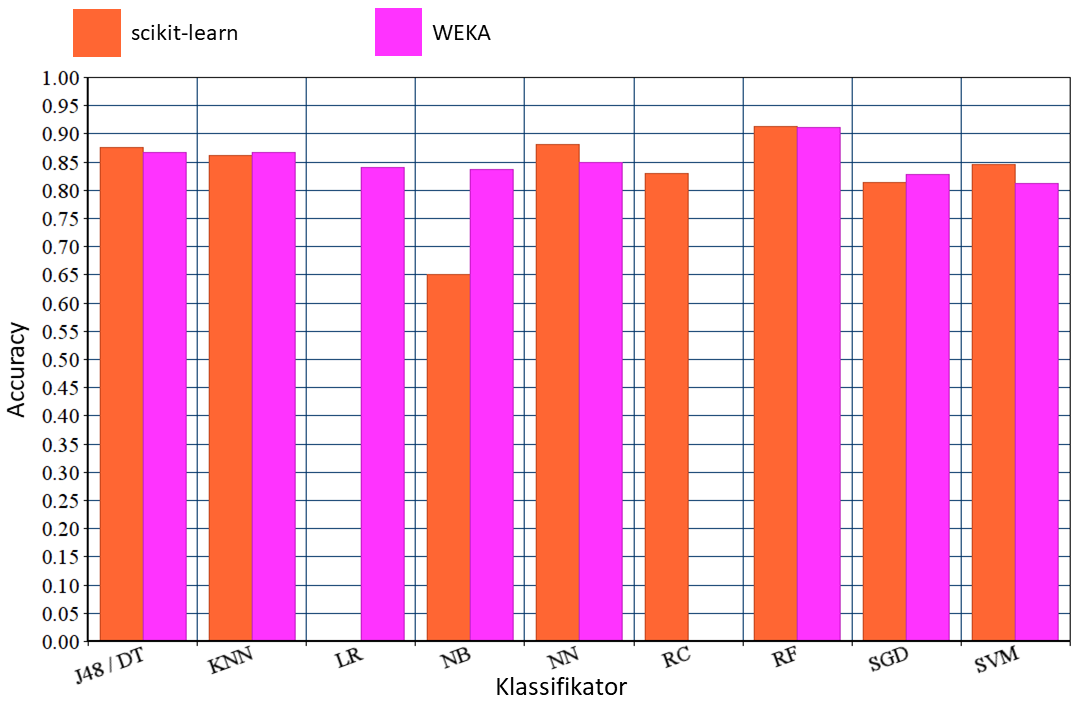
\includegraphics[width=\textwidth]{images/feat_final}
    \caption{Vergleich der Accuracies des featurebasierten Datensets\label{fig:final-feat}}
\end{figure}

\begin{figure}[t]
    \centering
    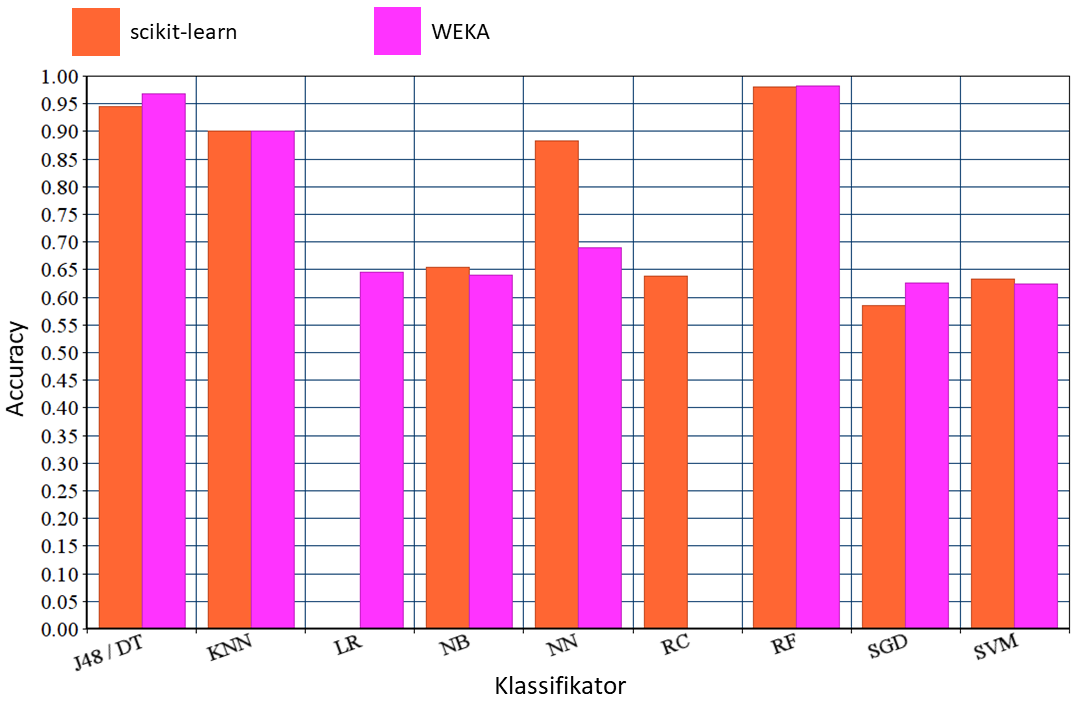
\includegraphics[width=\textwidth]{images/file_final}
    \caption{Vergleich der Accuracies des dateibasierten Datensets\label{fig:final-file}}
\end{figure}

\subsubsection*{Weitere Evaluationsmetriken}

Dieser Abschnitt stellt die Ergebnisse der weiteren Evaluationsmetriken TP-Rate / Recall, FP-Rate, Precision und F-Score vor. Diese können in \autoref{tab:met-feat} für das featurebasierte Datenset und in \autoref{tab:met-file} für das dateibasierte Datenset eingesehen werden. Aufgeteilt werden die Ergebnisse nach verwendetem Tool sowie nach den Werten der Zielklasse \glqq fehlerfrei\grqq{} und \glqq defekt\grqq. Zudem wird das gewichtete Mittel angegeben. Dabei handelt es sich um den Mittelwert der Ergebnisse beider Werte der Zielklasse unter Einbezug der Anzahl der korrekten Vorhersagen je Wert. Es zeigt somit die Performanz aggregiert für beide Werte an und liegt im Idealfall bei 1,00. Die vollständigen Tabellen der Ergebnisse der Evaluation, inklusive einer weiteren Metrik, können im \hyperref[appendix3]{Anhang} gefunden werden.

Betrachtet man die Ergebnisse der Metriken des featurebasierten Datensets in \autoref{tab:met-feat}, so ergibt sich eine breite Streuung der Werte. Jeder Klassifikator zeigt durch seine Ergebnisse seine individuellen \glqq Stärken\grqq{} und \glqq Schwächen\grqq. In der Gesamtheit der Kombination der Werte betrachtet, 

TOP: RF, KNN, DT (eingeschränkt)
Mittel: LR, NN
\textbf{NÄHER BETRACHTEN}


\begin{table}[t]
\centering
\caption{Ergebnisse der Evaluationsmetriken des featurebasierten Datensets}
\label{tab:met-feat}
\resizebox{\linewidth}{!}{%
\begin{tabular}{|>{\hspace{0pt}}p{0.085\linewidth}>{\hspace{0pt}}p{0.148\linewidth}|>{\RaggedLeft\hspace{0pt}}p{0.162\linewidth}>{\RaggedLeft\hspace{0pt}}p{0.114\linewidth}>{\RaggedLeft\hspace{0pt}}p{0.098\linewidth}|>{\RaggedLeft\hspace{0pt}}p{0.162\linewidth}>{\RaggedLeft\hspace{0pt}}p{0.114\linewidth}>{\RaggedLeft\hspace{0pt}}p{0.102\linewidth}|} 
\cline{3-8}
\multicolumn{1}{>{\hspace{0pt}}p{0.085\linewidth}}{}                                         &           & \multicolumn{3}{>{\Centering\hspace{0pt}}p{0.374\linewidth}|}{\textbf{scikit-learn} } & \multicolumn{3}{>{\Centering\hspace{0pt}}p{0.378\linewidth}|}{\textbf{WEKA} }  \\ 
\cline{3-8}
\multicolumn{1}{>{\hspace{0pt}}p{0.085\linewidth}}{}                                         &           & \textbf{Fehlerfrei}  & \textbf{Defekt}  & \textbf{gew.}\par{}\textbf{Mittel}          & \textbf{Fehlerfrei}  & \textbf{Defekt}  & \textbf{gew.}\par{}\textbf{Mittel}   \\ 
\hline
\multirow{4}{0.085\linewidth}{\hspace{0pt}\begin{tabular}[c]{@{}l@{}}DT /\\J48\end{tabular}} & TP-Rate   & 0,93                 & 0,65             & 0,88                                        & 0,95                 & 0,54             & 0,87                                 \\
                                                                                             & FP-Rate   & 0,65                 & 0,07             & 0,18                                        & 0,46                 & 0,05             & 0,38                                 \\
                                                                                             & Precision & 0,92                 & 0,69             & 0,87                                        & 0,89                 & 0,71             & 0,86                                 \\
                                                                                             & F-Score   & 0,92                 & 0,67             & 0,87                                        & 0,92                 & 0,62             & 0,86                                 \\ 
\hline
\multirow{4}{0.085\linewidth}{\hspace{0pt}KNN}                                               & TP-Rate   & 0,92                 & 0,62             & 0,86                                        & 0,93                 & 0,60             & 0,87                                 \\
                                                                                             & FP-Rate   & 0,62                 & 0,08             & 0,18                                        & 0,40                 & 0,07             & 0,33                                 \\
                                                                                             & Precision & 0,91                 & 0,63             & 0,86                                        & 0,91                 & 0,63             & 0,86                                 \\
                                                                                             & F-Score   & 0,92                 & 0,63             & 0,86                                        & 0,92                 & 0,64             & 0,86                                 \\ 
\hline
\multirow{4}{0.085\linewidth}{\hspace{0pt}LR}                                                & TP-Rate   &                      &                  &                                             & 0,98                 & 0,25             & 0,84                                 \\
                                                                                             & FP-Rate   &                      &                  &                                             & 0,75                 & 0,02             & 0,60                                 \\
                                                                                             & Precision &                      &                  &                                             & 0,84                 & 0,80             & 0,83                                 \\
                                                                                             & F-Score   &                      &                  &                                             & 0,91                 & 0,39             & 0,81                                 \\ 
\hline
\multirow{4}{0.085\linewidth}{\hspace{0pt}NB}                                                & TP-Rate   & 0,79                 & 0,07             & 0,65                                        & 0,98                 & 0,24             & 0,84                                 \\
                                                                                             & FP-Rate   & 0,07                 & 0,21             & 0,18                                        & 0,76                 & 0,02             & 0,61                                 \\
                                                                                             & Precision & 0,78                 & 0,07             & 0,64                                        & 0,81                 & 0,77             & 0,83                                 \\
                                                                                             & F-Score   & 0,79                 & 0,07             & 0,65                                        & 0,91                 & 0,37             & 0,80                                 \\ 
\hline
\multirow{4}{0.085\linewidth}{\hspace{0pt}NN}                                                & TP-Rate   & 0,94                 & 0,57             & 0,88                                        & 0,95                 & 0,46             & 0,85                                 \\
                                                                                             & FP-Rate   & 0,57                 & 0,06             & 0,07                                        & 0,54                 & 0,05             & 0,44                                 \\
                                                                                             & Precision & 0,91                 & 0,68             & 0,87                                        & 0,87                 & 0,70             & 0,84                                 \\
                                                                                             & F-Score   & 0,93                 & 0,92             & 0,88                                        & 0,91                 & 0,56             & 0,84                                 \\ 
\hline
\multirow{4}{0.085\linewidth}{\hspace{0pt}RC}                                                & TP-Rate   & 1,00                 & 0,10             & 0,83                                        &                      &                  &                                      \\
                                                                                             & FP-Rate   & 0,10                 & 0,00             & 0,02                                        &                      &                  &                                      \\
                                                                                             & Precision & 0,83                 & 0,89             & 0,84                                        &                      &                  &                                      \\
                                                                                             & F-Score   & 0,91                 & 0,18             & 0,77                                        &                      &                  &                                      \\ 
\hline
\multirow{4}{0.085\linewidth}{\hspace{0pt}RF}                                                & TP-Rate   & 0,97                 & 0,67             & 0,91                                        & 0,97                 & 0,67             & 0,91                                 \\
                                                                                             & FP-Rate   & 0,67                 & 0,03             & 0,15                                        & 0,33                 & 0,03             & 0,27                                 \\
                                                                                             & Precision & 0,93                 & 0,82             & 0,91                                        & 0,92                 & 0,87             & 0,91                                 \\
                                                                                             & F-Score   & 0,95                 & 0,74             & 0,91                                        & 0,95                 & 0,75             & 0,91                                 \\ 
\hline
\multirow{4}{0.085\linewidth}{\hspace{0pt}SGD}                                               & TP-Rate   & 0,95                 & 0,23             & 0,81                                        & 0,99                 & 0,15             & 0,93                                 \\
                                                                                             & FP-Rate   & 0,23                 & 0,05             & 0,09                                        & 0,85                 & 0,01             & 0,68                                 \\
                                                                                             & Precision & 0,84                 & 0,49             & 0,78                                        & 0,83                 & 0,87             & 0,84                                 \\
                                                                                             & F-Score   & 0,89                 & 0,32             & 0,81                                        & 0,90                 & 0,26             & 0,78                                 \\ 
\hline
\multirow{4}{0.085\linewidth}{\hspace{0pt}SVM}                                               & TP-Rate   & 0,99                 & 0,24             & 0,85                                        & 1,00                 & 0,04             & 0,81                                 \\
                                                                                             & FP-Rate   & 0,24                 & 0,01             & 0,06                                        & 0,96                 & 0,00             & 0,77                                 \\
                                                                                             & Precision & 0,85                 & 0,80             & 0,84                                        & 0,81                 & 0,96             & 0,84                                 \\
                                                                                             & F-Score   & 0,91                 & 0,37             & 0,81                                        & 0,90                 & 0,08             & 0,74                                 \\
\hline
\end{tabular}
}
\end{table}

\begin{table}[t]
\centering
\caption{Ergebnisse der Evaluationsmetriken des dateibasierten Datensets}
\label{tab:met-file}
\resizebox{\linewidth}{!}{%
\begin{tabular}{|>{\hspace{0pt}}p{0.087\linewidth}>{\hspace{0pt}}p{0.15\linewidth}|>{\RaggedLeft\hspace{0pt}}p{0.156\linewidth}>{\RaggedLeft\hspace{0pt}}p{0.114\linewidth}>{\RaggedLeft\hspace{0pt}}p{0.102\linewidth}|>{\RaggedLeft\hspace{0pt}}p{0.156\linewidth}>{\RaggedLeft\hspace{0pt}}p{0.116\linewidth}>{\RaggedLeft\hspace{0pt}}p{0.104\linewidth}|} 
\cline{3-8}
\multicolumn{1}{>{\hspace{0pt}}p{0.087\linewidth}}{ \textbf{} }                              & \textbf{}  & \multicolumn{3}{>{\Centering\hspace{0pt}}p{0.372\linewidth}|}{\textbf{scikit-learn} } & \multicolumn{3}{>{\Centering\hspace{0pt}}p{0.376\linewidth}|}{\textbf{WEKA} }  \\ 
\cline{3-8}
\multicolumn{1}{>{\Centering\hspace{0pt}}p{0.087\linewidth}}{}                               &            & \textbf{fehlerfrei}  & \textbf{defekt}  & \textbf{gew.}\par{}\textbf{Mittel}          & \textbf{fehlerfrei}  & \textbf{defekt}  & \textbf{gew.}\par{}\textbf{Mittel}   \\ 
\hline
\multirow{4}{0.087\linewidth}{\hspace{0pt}\begin{tabular}[c]{@{}l@{}}DT /\\J48\end{tabular}} & TP-Rate    & 0,99                 & 0,87             & 0,94                                        & 0,98                 & 0,95             & 0,97                                 \\
                                                                                             & FP-Rate    & 0,87                 & 0,01             & 0,35                                        & 0,05                 & 0,02             & 0,03                                 \\
                                                                                             & Precision  & 0,92                 & 0,99             & 0,95                                        & 0,97                 & 0,97             & 0,97                                 \\
                                                                                             & F-Score    & 0,96                 & 0,93             & 0,94                                        & 0,97                 & 0,96             & 0,97                                 \\ 
\hline
\multirow{4}{0.087\linewidth}{\hspace{0pt}KNN}                                               & TP-Rate    & 0,89                 & 0,91             & 0,90                                        & 0,92                 & 0,87             & 0,90                                 \\
                                                                                             & FP-Rate    & 0,91                 & 0,11             & 0,43                                        & 0,13                 & 0,08             & 0,11                                 \\
                                                                                             & Precision  & 0,94                 & 0,85             & 0,90                                        & 0,91                 & 0,88             & 0,90                                 \\
                                                                                             & F-Score    & 0,92                 & 0,88             & 0,90                                        & 0,92                 & 0,88             & 0,90                                 \\ 
\hline
\multirow{4}{0.087\linewidth}{\hspace{0pt}LR}                                                & TP-Rate    &                      &                  &                                             & 0,92                 & 0,24             & 0,65                                 \\
                                                                                             & FP-Rate    &                      &                  &                                             & 0,76                 & 0,08             & 0,49                                 \\
                                                                                             & Precision  &                      &                  &                                             & 0,64                 & 0,66             & 0,65                                 \\
                                                                                             & F-Score    &                      &                  &                                             & 0,76                 & 0,36             & 0,60                                 \\ 
\hline
\multirow{4}{0.087\linewidth}{\hspace{0pt}NB}                                                & TP-Rate    & 0,66                 & 0,64             & 0,65                                        & 0,87                 & 0,30             & 0,64                                 \\
                                                                                             & FP-Rate    & 0,64                 & 0,34             & 0,46                                        & 0,70                 & 0,13             & 0,47                                 \\
                                                                                             & Precision  & 0,73                 & 0,56             & 0,66                                        & 0,65                 & 0,61             & 0,63                                 \\
                                                                                             & F-Score    & 0,70                 & 0,60             & 0,66                                        & 0,74                 & 0,40             & 0,60                                 \\ 
\hline
\multirow{4}{0.087\linewidth}{\hspace{0pt}NN}                                                & TP-Rate    & 0,97                 & 0,76             & 0,88                                        & 0,86                 & 0,41             & 0,68                                 \\
                                                                                             & FP-Rate    & 0,76                 & 0,03             & 0,33                                        & 0,59                 & 0,14             & 0,41                                 \\
                                                                                             & Precision  & 0,86                 & 0,94             & 0,89                                        & 0,69                 & 0,67             & 0,68                                 \\
                                                                                             & F-Score    & 0,91                 & 0,84             & 0,88                                        & 0,76                 & 0,51             & 0,66                                 \\ 
\hline
\multirow{4}{0.087\linewidth}{\hspace{0pt}RC}                                                & TP-Rate    & 0,92                 & 0,23             & 0,64                                        &                      &                  &                                      \\
                                                                                             & FP-Rate    & 0,23                 & 0,08             & 0,14                                        &                      &                  &                                      \\
                                                                                             & Precision  & 0,63                 & 0,66             & 0,64                                        &                      &                  &                                      \\
                                                                                             & F-Score    & 0,75                 & 0,34             & 0,58                                        &                      &                  &                                      \\ 
\hline
\multirow{4}{0.087\linewidth}{\hspace{0pt}RF}                                                & TP-Rate    & 0,99                 & 0,97             & 0,98                                        & 0,99                 & 0,97             & 0,98                                 \\
                                                                                             & FP-Rate    & 0,97                 & 0,01             & 0,40                                        & 0,03                 & 0,01             & 0,02                                 \\
                                                                                             & Precision  & 0,98                 & 0,98             & 0,98                                        & 0,98                 & 0,99             & 0,98                                 \\
                                                                                             & F-Score    & 0,98                 & 0,98             & 0,98                                        & 0,99                 & 0,98             & 0,98                                 \\ 
\hline
\multirow{4}{0.087\linewidth}{\hspace{0pt}SGD}                                               & TP-Rate    & 0,67                 & 0,45             & 0,58                                        & 0,97                 & 0,12             & 0,63                                 \\
                                                                                             & FP-Rate    & 0,45                 & 0,33             & 0,38                                        & 0,88                 & 0,03             & 0,54                                 \\
                                                                                             & Precision  & 0,65                 & 0,48             & 0,58                                        & 0,62                 & 0,71             & 0,66                                 \\
                                                                                             & F-Score    & 0,66                 & 0,47             & 0,58                                        & 0,76                 & 0,20             & 0,53                                 \\ 
\hline
\multirow{4}{0.087\linewidth}{\hspace{0pt}SVM}                                               & TP-Rate    & 0,93                 & 0,20             & 0,63                                        & 0,97                 & 0,11             & 0,62                                 \\
                                                                                             & FP-Rate    & 0,20                 & 0,07             & 0,12                                        & 0,89                 & 0,03             & 0,55                                 \\
                                                                                             & Precision  & 0,63                 & 0,65             & 0,64                                        & 0,62                 & 0,69             & 0,65                                 \\
                                                                                             & F-Score    & 0,75                 & 0,31             & 0,57                                        & 0,75                 & 0,19             & 0,53                                 \\
\hline
\end{tabular}
}
\end{table}

\subsubsection*{ROC-Kurven und ROC-Bereiche}

Die Interpretation der ROC-Kurven und ROC-Bereiche erfolgt anhand des in \hyperref[roc-def]{Abschnitt 5.2.1} vorgestellten Schemas. Die ROC-Kurven samt der Werte der ROC-Bereiche (repräsentiert durch \glqq AUC\grqq) sind in \autoref{fig:roc-feat} (featurebasiertes Datenset) und \autoref{fig:roc-file} dargestellt. Zu sehen sind jeweils die von den Tools scikit-learn und WEKA ausgegebenen und unveränderten Plots. Die in den Plots des Tools WEKA dargestellten Farbverläufe der Kurven verdeutlichen keine für diesen Zweck relevanten Informationen und können somit ignoriert werden.

Die ROC-Kurven des featurebasierten Datensets in \autoref{fig:roc-feat} zeigen, dass erneut der Ent-scheidungsbaum-basierte Klassifikator RF beider Tools nahezu den Idealfall der Performanz widerspiegeln. Dies bezeugen auch die ROC-Bereiche von 0,95. Die Klassifikatoren SGD und SVM (nur WEKA) zeigen hingegen den nahezu schlechtesten Fall mit winkelhalbierenden Kurven und ROC-Bereichen nahe des unerwünschten Wertes von 0,50. Dies zeigt, dass die Klassifikatoren die Werte der Zielklasse nicht unterscheiden können und somit \glqq raten\grqq{} statt präzise vorherzusagen. Eine weitere Besonderheit stellt die ROC-Kurve des NB-Klassifikators von scikit-learn dar. Sie verläuft konvex und besitzt einen ROC-Bereich von 0,41, welcher unter dem unerwünschten Wert liegt. Dies bedeutet, dass der Klassifikator inverse Vorhersagen trifft. Im vorliegenden Fall bedeutet dies, dass statt dem Label \glqq fehlerfrei\grqq{} das inverse, also gegenteilige, Label \glqq defekt\grqq{} vorhersagt wird. Für den Fall eines ROC-Bereiches von 0,00 können somit die Label einfach invertiert werden. Die weiteren Klassifikatoren besitzen ROC-Kurven, welche den Normalfall mit einer durchschnittlichen oder überdurchschnittlichen Performanz darstellen. Der Vergleich zwischen den verwendeten Tools zeigt, dass sich die Kurven und die Werte der Bereiche in den überwiegenden Fällen ähneln. Lediglich die Klassifikatoren NB und SVM weisen signifikante Unterschiede auf. Begründet werden kann dies durch verschiedene Implementierungsansätze der Klassifikationsalgorithmen in den Tools. So ist zum Beispiel nicht ersichtlich, welche Variation des NB-Klassifikators von WEKA verwendet wird. Diese kann somit gegebenenfalls nicht für die zugrundeliegenden Datensets optimiert sein und zu ungenauen oder falschen Ergebnissen führen.

Der Blick auf die ROC-Kurven des dateibasierten Datensets in \autoref{fig:roc-file} zeigt, dass die Performanzen, gegenüber des featurebasierten Datensets, für die meisten Klassifikatoren höher ausfallen. Insbesondere die Klassifikatoren, welche in der ersten und zweiten Zeile der Abbildung dargestellt sind, mit Ausnahme des NN-Klassifikators von WEKA, besitzen ROC-Kurven, die nahezu oder vollständig dem Idealfall entsprechen. Die jeweiligen ROC-Bereiche mit Werten von über 0,90 bekräftigen dies. Einbußen in der Performanz können, mit Ausnahme des NB-Klassifikators von scikit-learn, bei den Klassifikatoren der dritten und vierten Zeile festgestellt werden. Keiner der Klassifikatoren konnte einen ROC-Bereich von 0,70 erreichen. Ihre Leistung ist somit auf ein unterdurchschnittliches Niveau gesunden. Die WEKA-Klassifikatoren SGD und SVM zeigen weiterhin den unerwünschten Fall.

Auch die Betrachtung der ROC-Kurven mit ihren zugehörigen Bereichen zeigte erneut, dass die RF-Klassifikatoren die beste Wahl für den in dieser Arbeit vorliegenden Klassifikationsfall darstellen. Sie zeigten in allen Gesichtspunkten der Evaluation die höchste Performanz.

\begin{figure}[t]
  \centering
  \subfloat[][DT (scikit) \\AUC = 0,79]{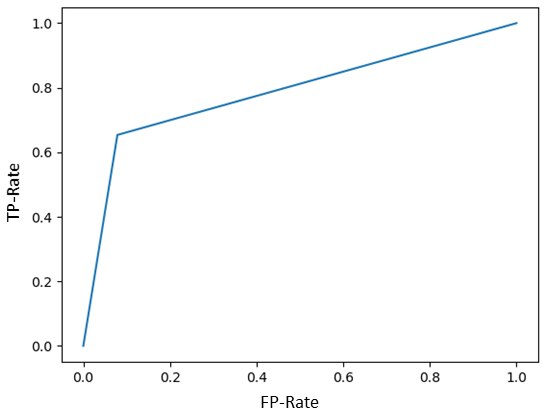
\includegraphics[width=0.25\linewidth]{images/dt_scikit}}
  \subfloat[][J48 (WEKA)\\AUC = 0,88]{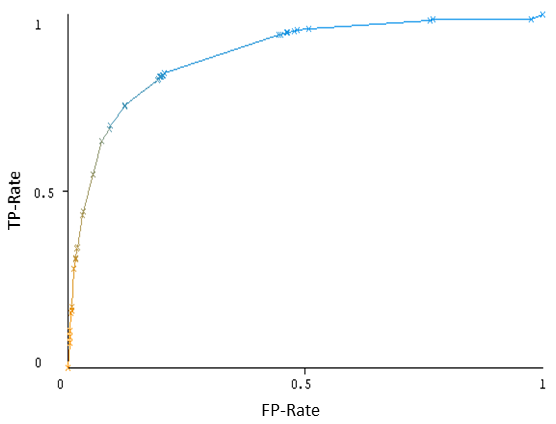
\includegraphics[width=0.25\linewidth]{images/j48_weka}}
  \subfloat[][NN (scikit)\\AUC = 0,89]{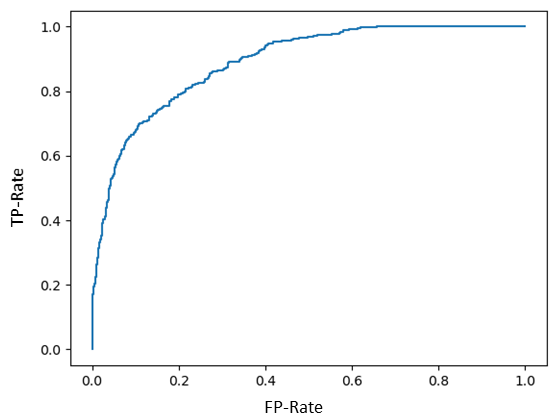
\includegraphics[width=0.25\linewidth]{images/nn_scikit}}
  \subfloat[][NN (WEKA)\\ AUC = 0,86]{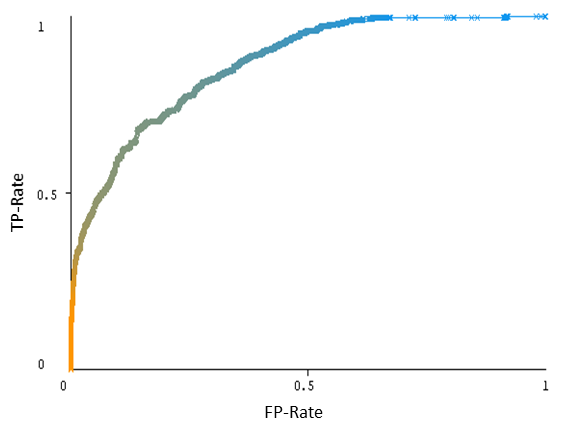
\includegraphics[width=0.25\linewidth]{images/nn_weka}}
  \qquad
  \subfloat[][KNN (scikit)\\AUC = 0,77]{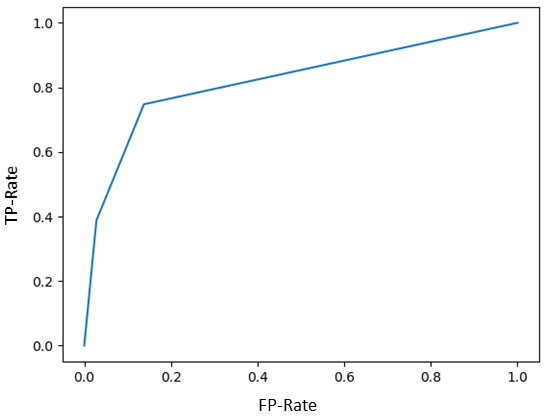
\includegraphics[width=0.25\linewidth]{images/knn_scikit}}
  \subfloat[][KNN (WEKA)\\AUC = 0,85]{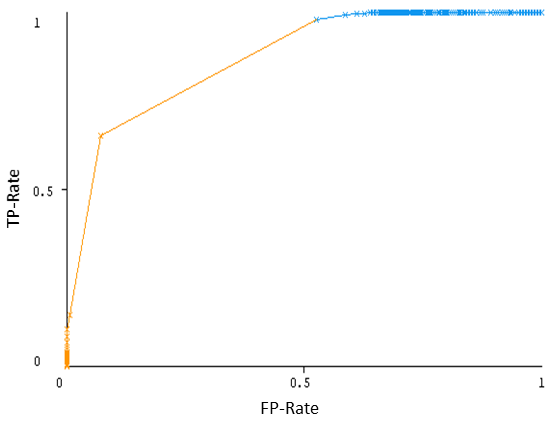
\includegraphics[width=0.25\linewidth]{images/knn_weka}}
  \subfloat[][RF (scikit)\\AUC = 0,95]{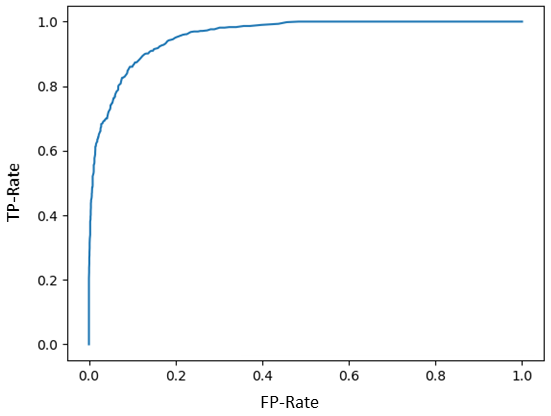
\includegraphics[width=0.25\linewidth]{images/rf_scikit}}
  \subfloat[][RF (WEKA)\\AUC = 0,95]{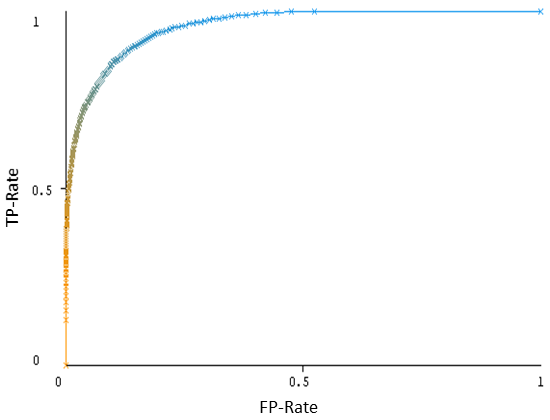
\includegraphics[width=0.25\linewidth]{images/rf_weka}}
  \qquad
  \subfloat[][RC (scikit)\\AUC = 0,77]{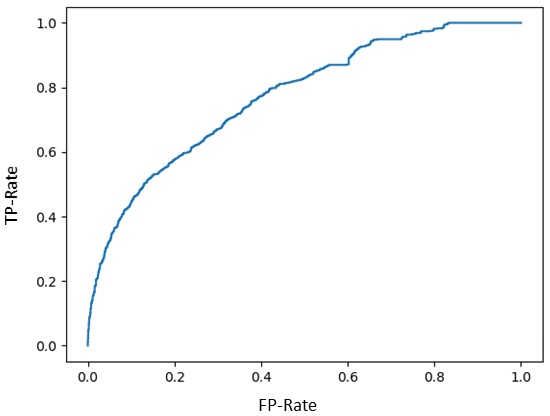
\includegraphics[width=0.25\linewidth]{images/rc_scikit}}
  \subfloat[][LR (WEKA)\\AUC = 0,82]{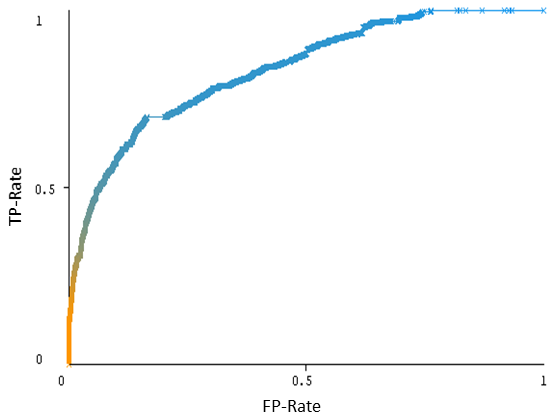
\includegraphics[width=0.25\linewidth]{images/lr_weka}}
  \subfloat[][SGD (scikit)\\AUC = 0,59]{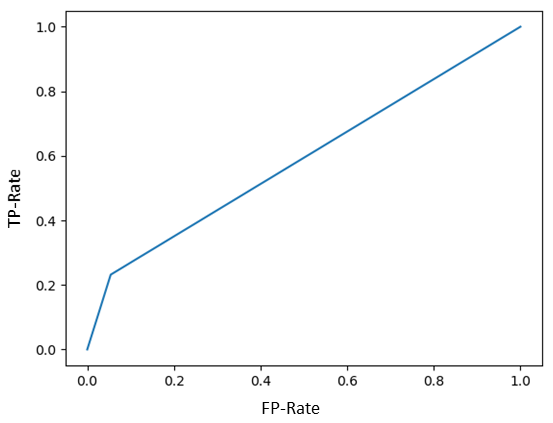
\includegraphics[width=0.25\linewidth]{images/sgd_scikit}}
  \subfloat[][SGD (WEKA)\\AUC = 0,57]{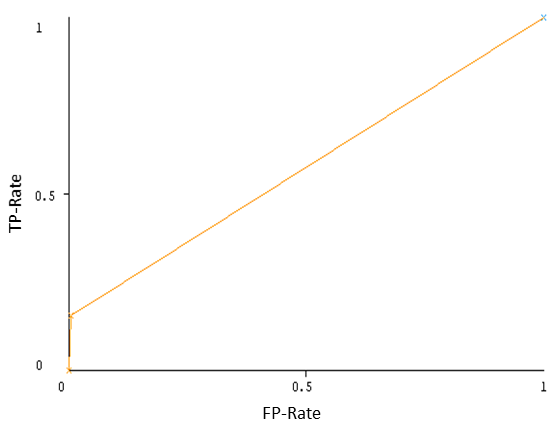
\includegraphics[width=0.25\linewidth]{images/sgd_weka}}
  \qquad
  \subfloat[][NB (scikit)\\AUC = 0,41]{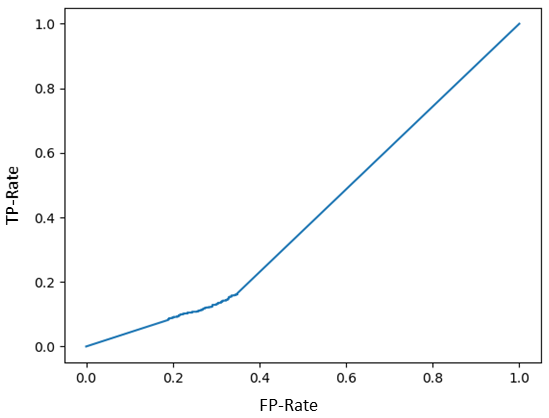
\includegraphics[width=0.25\linewidth]{images/nb_scikit}}
  \subfloat[][NB (WEKA)\\AUC = 0,74]{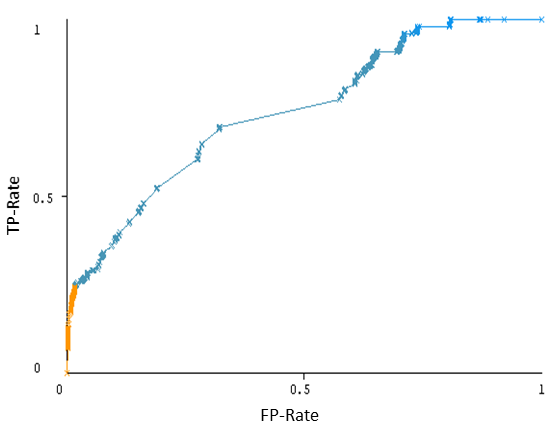
\includegraphics[width=0.25\linewidth]{images/nb_weka}}
  \subfloat[][SVM (scikit)\\AUC = 0,81]{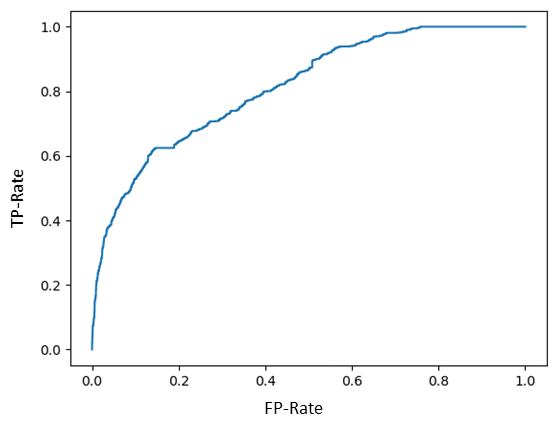
\includegraphics[width=0.25\linewidth]{images/svm_scikit}}
  \subfloat[][SVM (WEKA)\\AUC = 0,52]{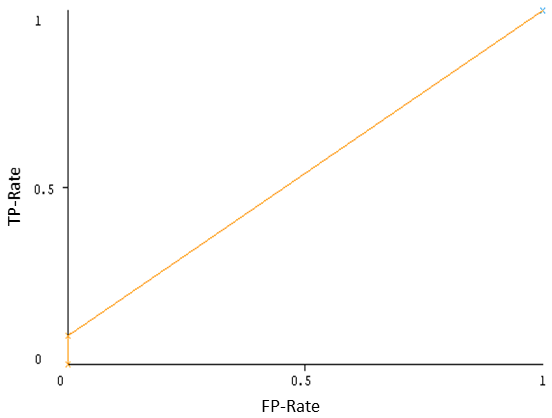
\includegraphics[width=0.25\linewidth]{images/svm_weka}}
  \caption{ROC-Kurven der Klassifikatoren des featurebasierten Datensets \label{fig:roc-feat}}
\end{figure}

\begin{figure}[t]
  \centering
  \subfloat[][DT (scikit)\\AUC = 0,94]{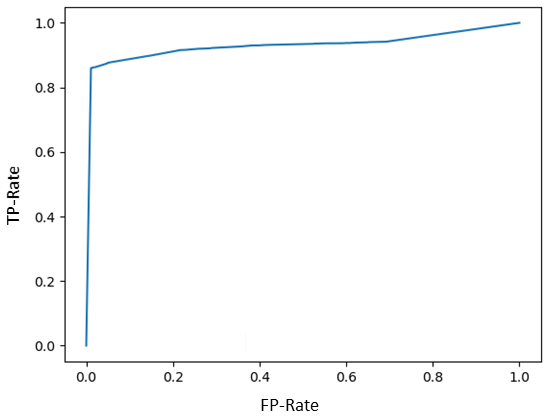
\includegraphics[width=0.25\linewidth]{images/dt_scikit_file}}
  \subfloat[][J48 (WEKA)\\AUC = 0,98]{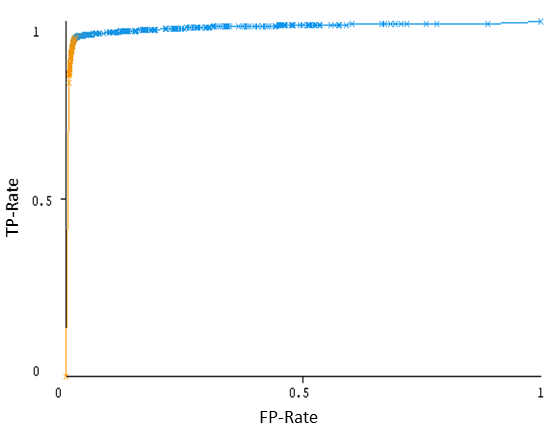
\includegraphics[width=0.25\linewidth]{images/j48_weka_file}}
  \subfloat[][NN (scikit)\\AUC = 0,95]{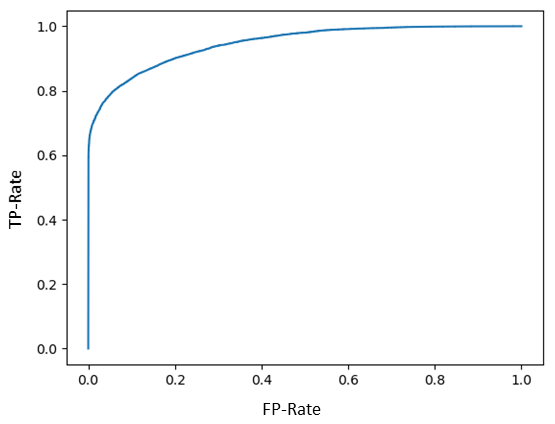
\includegraphics[width=0.25\linewidth]{images/nn_scikit_file}}
  \subfloat[][NN (WEKA)\\AUC = 0,73]{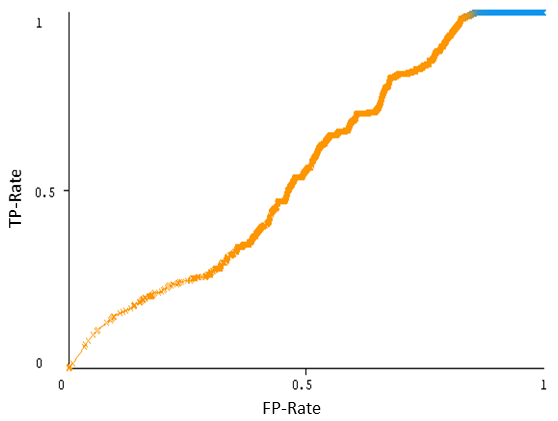
\includegraphics[width=0.25\linewidth]{images/nn_weka_file}}
  \qquad
  \subfloat[][KNN (scikit)\\AUC = 0,90]{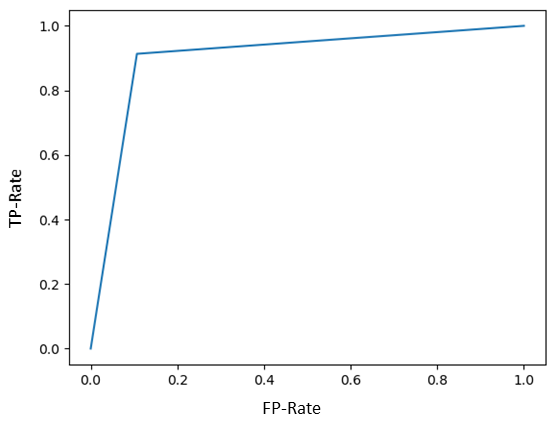
\includegraphics[width=0.25\linewidth]{images/knn_scikit_file}}
  \subfloat[][KNN (WEKA)\\AUC = 0,91]{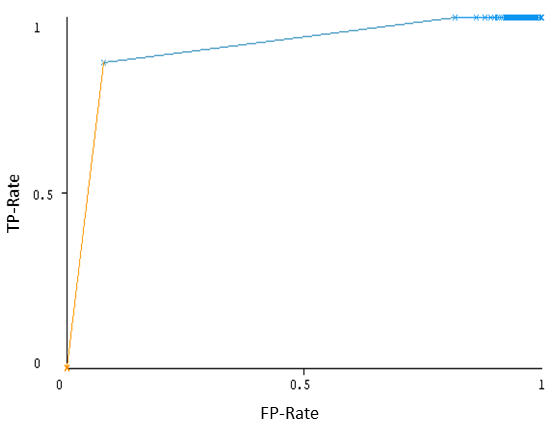
\includegraphics[width=0.25\linewidth]{images/knn_weka_file}}
  \subfloat[][RF (scikit)\\AUC = 1,00]{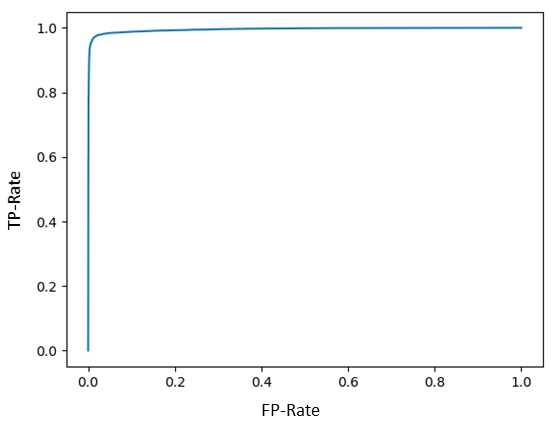
\includegraphics[width=0.25\linewidth]{images/rf_scikit_file}}
  \subfloat[][RF (WEKA)\\AUC = 1,00]{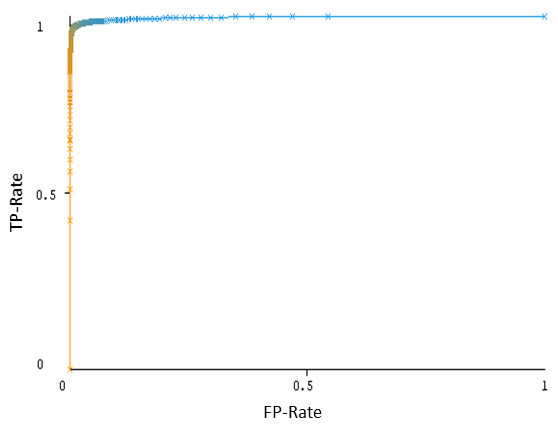
\includegraphics[width=0.25\linewidth]{images/rf_weka_file}}
  \qquad
  \subfloat[][RC (scikit)\\AUC = 0,64]{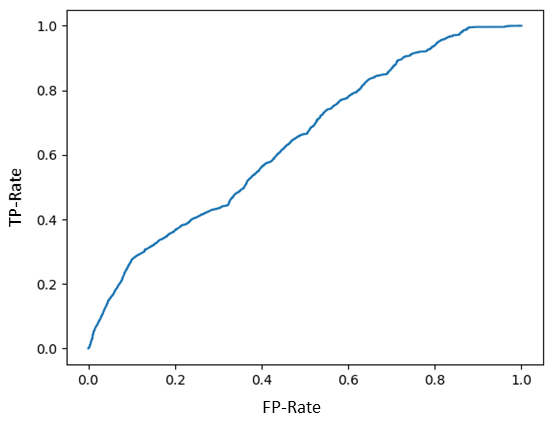
\includegraphics[width=0.25\linewidth]{images/rc_scikit_file}}
  \subfloat[][LR (WEKA)\\AUC = 0,67]{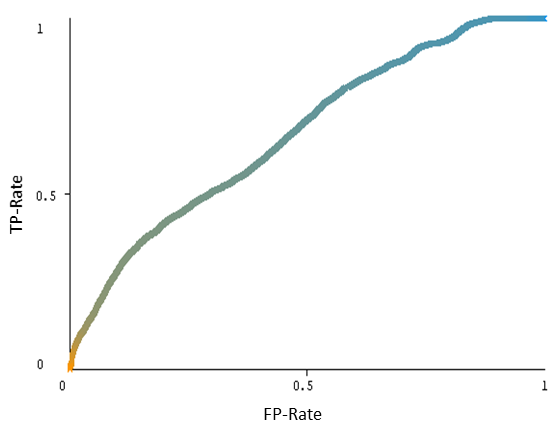
\includegraphics[width=0.25\linewidth]{images/lr_weka_file}}
  \subfloat[][SGD (scikit)\\AUC = 0,53]{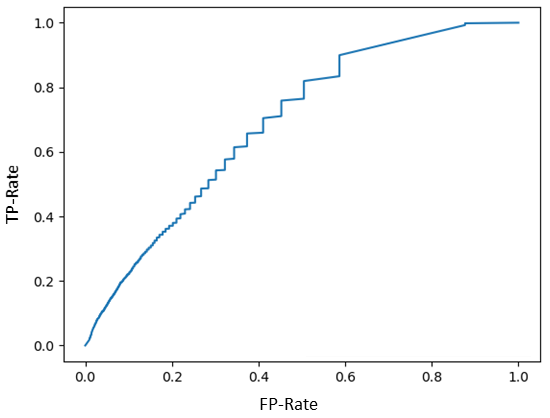
\includegraphics[width=0.25\linewidth]{images/sgd_scikit_file}}
  \subfloat[][SGD (WEKA)\\AUC = 0,54]{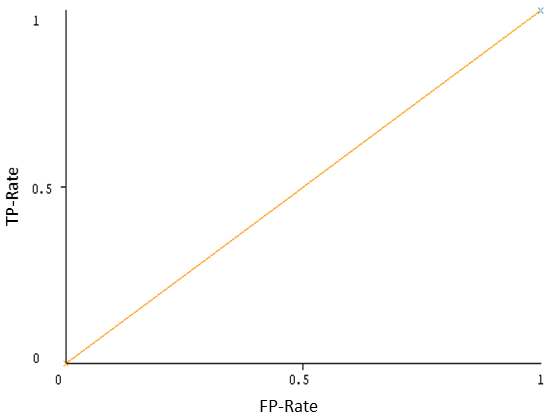
\includegraphics[width=0.25\linewidth]{images/sgd_weka_file}}
  \qquad
  \subfloat[][NB (scikit)\\AUC = 0,69]{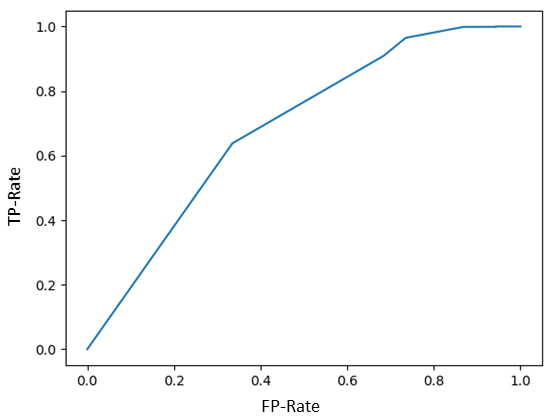
\includegraphics[width=0.25\linewidth]{images/nb_scikit_file}}
  \subfloat[][NB (WEKA)\\AUC = 0,64]{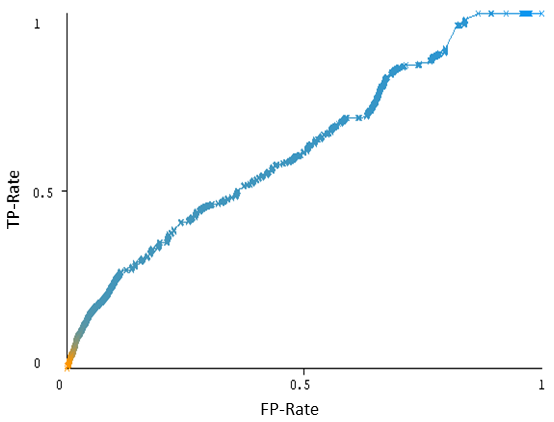
\includegraphics[width=0.25\linewidth]{images/nb_weka_file}}
  \subfloat[][SVM (scikit)\\AUC = 0,65]{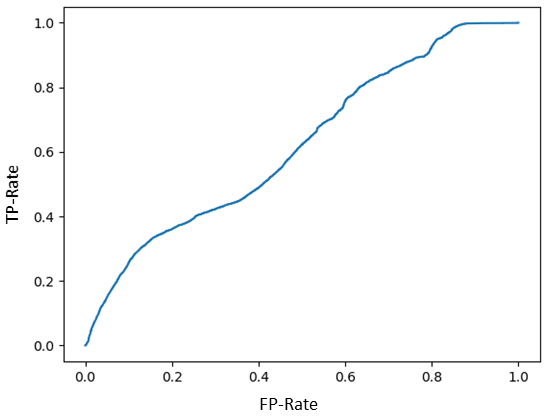
\includegraphics[width=0.25\linewidth]{images/svm_scikit_file}}
  \subfloat[][SVM (WEKA)\\AUC = 0,54]{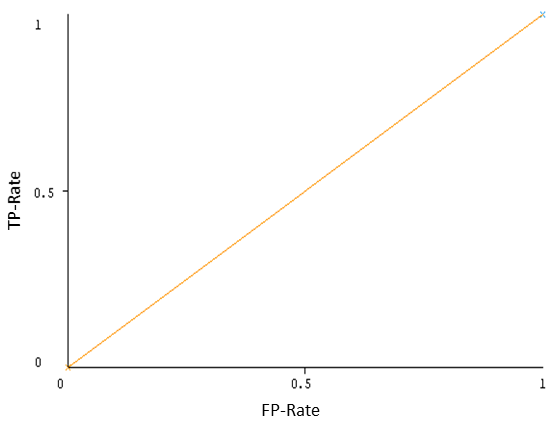
\includegraphics[width=0.25\linewidth]{images/svm_weka_file}}
  \caption{ROC-Kurven der Klassifikatoren des dateibasierten Datensets \label{fig:roc-file}}
\end{figure}

\fbox{\parbox{\linewidth}{RQ3c: WELCHE VOR- UND NACHTEILE BESITZT EIN KLASSIFIKATOR?\medskip\\
Hier soll mal so viel Text stehen, damit der ganze Text nicht nur in einer Zeile steht sondern in mindestens zwei oder mehr Zeilen, denn andernfalls werden wir nicht sehen können ob der Rahmen nur um die erste Zeile geht, oder wie wir wollen sich um den ganzen Absatz zieht.}}

\section{Vergleich zu nicht-featurebasierten Methoden}
\label{classic-eval}

Zum besseren Vergleich der Ergebnisse des Datensets mit neuartiger Fokussierung auf Software-Features, wird nicht nur das unter Zuhilfenahme der gleichen Metriken erstellte dateibasierte Datensets hinzugezogen, sondern zusätzlich ein Datenset, dessen Erstellung aus der wissenschaftlichen Literatur entnommen wurde und sich ebenfalls dem gängigen Weg der dateibasierten Fehlervorhersage widmet. Die von Moser et al. vorgestellte Methode umfasst die Berechnung von 17 Prozessmetriken, welche in \autoref{tab:eval-metrics} aufgeführt sind \cite{Moser2008}. Die Grundlage der Berechnungen bildeten die aus den Software-Repositories mittels PyDriller erhaltenen Daten. Zur Berechnung der \texttt{REVISIONS}-Metrik wurden die Commit-Nachrichten, analog zur Identifikation der fehlerbehebenden Commits, auf das Vorhandensein des Schlagwortes \glqq refactor\grqq{} analysiert. Zur Berechnung der Metriken \texttt{AGE} und \texttt{WEIGHTED\_AGE} wurde zudem für jeden Commit das zugehörige Datum der Ausführung abgerufen. Die Berechnung erfolgte entweder direkt mittels SQL-Abrufen oder mithilfe von Python-Skripten. Aufgrund der Unbalanciertheit des Datensets wurde der SMOTE-Algorithmus mit einem Wert von 3000 angewendet.

Zur besseren Vergleichbarkeit dieses Ansatzes, wurden die Metriken für ein weiteres Datenset unter Berücksichtigung des Feature-Aspekts berechnet. Dieses Datenset basiert ebenfalls aus den mit PyDriller erhaltenen Rohdaten und beinhaltet nur jede Dateien, in welchen ein Feature entfernt, hinzugefügt oder verändert wurde. Im weiteren Verlauf des Abschnitts wird dieses Datenset als \glqq vorhandenes Datenset\grqq{} bezeichnet, welches ebenfalls mit dem SMOTE-Algorithmus mit einem Wert von 300 erweitert wurde.

\begin{table}[t]
\centering
\caption{Übersicht der berechneten Metriken nach \cite{Moser2008}}
\label{tab:eval-metrics}
\resizebox{\textwidth}{!}{%
\begin{tabular}{|l|c|l|}
\hline
\textbf{Name}     & \textbf{Abkürzung} & \textbf{Beschreibung}                                                                                                                                                                                            \\ \hline
REVISIONS         & revi               & Anzahl der Revisionen (Bearbeitungen) der Datei.                                                                                                                                                                 \\
REFACTORINGS      & refa               & \begin{tabular}[c]{@{}l@{}}Anzahl der Fälle, in denen die Datei in einem Refactoring\\ involviert war.  Basierend auf Analyse der Commit-Nachricht\\ auf das Vorhandensein des Begriffs "refactor".\end{tabular} \\
BUGFIXES          & bugf               & \begin{tabular}[c]{@{}l@{}}Anzahl der Fälle, in denen die Datei in einer Fehlerbehebung\\ involviert war.\end{tabular}                                                                                           \\
AUTHORS           & auth               & \begin{tabular}[c]{@{}l@{}}Anzahl der verschiedenen Autoren, die die Datei in das\\ Repository eingecheckt haben.\end{tabular}                                                                                   \\
LOC\_ADDED        & addl               & \begin{tabular}[c]{@{}l@{}}Summe der zur Datei hinzugefügten Codezeilen über\\ alle Revisionen.\end{tabular}                                                                                                     \\
MAX\_LOC\_ADDED   & addm               & \begin{tabular}[c]{@{}l@{}}Maximale Anzahl von Codezeilen, die für alle Revisionen\\ hinzugefügt wurden.\end{tabular}                                                                                            \\
AVE\_LOC\_ADDED   & adda               & Durchschnittlich hinzugefügte Codezeilen pro Revision.                                                                                                                                                           \\
LOC\_DELETED      & reml               & \begin{tabular}[c]{@{}l@{}}Summe der von der Datei entfernten Codezeilen über alle\\ Revisionen.\end{tabular}                                                                                                    \\
MAX\_LOC\_DELETED & remm               & \begin{tabular}[c]{@{}l@{}}Maximale Anzahl von Codezeilen, die für alle Revisionen\\ entfernt wurden.\end{tabular}                                                                                               \\
AVE\_LOC\_DELETED & rema               & Durchschnittlich entfernte Codezeilen pro Revision.                                                                                                                                                              \\
CODECHURN         & cchl               & \begin{tabular}[c]{@{}l@{}}Summe von (hinzugefügte Codezeilen - entfernte Codezeilen)\\ über alle Revisionen.\end{tabular}                                                                                       \\
MAX\_CODECHURN    & cchl               & Maximaler CODECHURN für alle Revisionen.                                                                                                                                                                         \\
AVE\_CODECHURN    & ccha               & Durchschnittlicher CODECHURN pro Revision.                                                                                                                                                                       \\
MAX\_CHANGESET    & maxc               & \begin{tabular}[c]{@{}l@{}}Maximale Anzahl von Dateien, die gemeinsam committed\\ wurden.\end{tabular}                                                                                                           \\
AVE\_CHANGESET    & avgc               & \begin{tabular}[c]{@{}l@{}}Durchschnittliche Anzahl von Dateien, die gemeinsam\\ committed wurden.\end{tabular}                                                                                                  \\
AGE               & aage               & \begin{tabular}[c]{@{}l@{}}Alter der Datei in Wochen (rückwärts zählend bis zu\\ einem bestimmten Release).\end{tabular}                                                                                         \\
WEIGHTED\_AGE     & wage               & $Weighted Age = \frac{\sum_{i=1}^N Age(i)*LOC\_ADDED(i)}{\sum_{i=1}^N LOC\_ADDED(i)}$                                                                                                                                                                                                           \\ \hline
\end{tabular}%
}
\end{table}

\fbox{\parbox{\linewidth}{RQ3d: WIE LASSEN SICH DIE KLASSIFIKATOREN MIT WEITEREN VORHERSAGETECHNIKEN, DIE KEINE FEATURES NUTZEN, VERGLEICHEN?\medskip\\
Es wurde auf eine Methode zur Erstellung eines dateibasierten Datensets aus der wissenschaftlichen Literatur zurückgegriffen \cite{Moser2008}. Dieses Datenset basiert auf den mittels PyDriller abgerufenen Daten und umfasst 17 Attribute. Zum besseren Vergleich wurde ein weiteres Datenset erstellt, welches nur jene Dateien umfasst, in denen sich Featurecode befindet.}}

\subsubsection*{Konfusionsmatrizen}

\begin{table}[t]
\centering
\caption{Konfusionsmatrizen des nicht-featurebasierten Vergleichs}
\label{tab:class-mat}
\resizebox{\linewidth}{!}{%
\begin{tabular}{|>{\hspace{0pt}}p{0.075\linewidth}>{\hspace{0pt}}p{0.229\linewidth}|>{\RaggedLeft\hspace{0pt}}p{0.145\linewidth}>{\RaggedLeft\hspace{0pt}}p{0.1\linewidth}>{\RaggedLeft\hspace{0pt}}p{0.1\linewidth}|>{\RaggedLeft\hspace{0pt}}p{0.145\linewidth}>{\RaggedLeft\hspace{0pt}}p{0.102\linewidth}>{\RaggedLeft\hspace{0pt}}p{0.089\linewidth}|} 
\cline{3-8}
\multicolumn{1}{>{\hspace{0pt}}p{0.075\linewidth}}{}            &                                    & \multicolumn{3}{>{\Centering\hspace{0pt}}p{0.345\linewidth}|}{\textbf{Datenset nach \cite{Moser2008}}} & \multicolumn{3}{>{\Centering\hspace{0pt}}p{0.335\linewidth}|}{\textbf{vorhandenes Datenset}}  \\ 
\cline{2-8}
\multicolumn{1}{>{\Centering\hspace{0pt}}p{0.075\linewidth}|}{} & \textbf{Ermittelt -\textgreater{}} & \textbf{Fehlerfrei}  & \textbf{Defekt}  & \textbf{Total}                              & \textbf{Fehlerfrei}  & \textbf{Defekt}  & \textbf{Total}                                      \\ 
\hline
\multirow{3}{0.075\linewidth}{\hspace{0pt}J48}                  & Realität fehlerfrei                & 12.845               & 233              & 13.078                                      & 2.378                & 191              & 2.569                                               \\
                                                                & Realität defekt                    & 394                  & 5.586            & 5.980                                       & 258                  & 597              & 855                                                 \\
                                                                & Total                              & 13.239               & 5.819            & 19.058                                      & 2.636                & 788              & 3.424                                               \\ 
\hline
\multirow{3}{0.075\linewidth}{\hspace{0pt}KNN}                  & Realität fehlerfrei                & 12.565               & 513              & 13.078                                      & 1.679                & 154              & 1.833                                               \\
                                                                & Realität defekt                    & 928                  & 5.052            & 5.980                                       & 242                  & 371              & 613                                                 \\
                                                                & Total                              & 13.493               & 5.565            & 19.058                                      & 1.921                & 525              & 2.446                                               \\ 
\hline
\multirow{3}{0.075\linewidth}{\hspace{0pt}LR}                   & Realität fehlerfrei                & 12.495               & 583              & 13.078                                      & 2.531                & 38               & 2.569                                               \\
                                                                & Realität defekt                    & 4.934                & 1.046            & 5.980                                       & 785                  & 70               & 855                                                 \\
                                                                & Total                              & 17.429               & 1.629            & 19.058                                      & 3.316                & 108              & 3.424                                               \\ 
\hline
\multirow{3}{0.075\linewidth}{\hspace{0pt}NB}                   & Realität fehlerfrei                & 6.224                & 15.485           & 21.709                                      & 28                   & 1.059            & 1.087                                               \\
                                                                & Realität defekt                    & 698                  & 9.356            & 10.054                                      & 15                   & 366              & 381                                                 \\
                                                                & Total                              & 6.922                & 24.841           & 31.763                                      & 43                   & 1.425            & 1.468                                               \\ 
\hline
\multirow{3}{0.075\linewidth}{\hspace{0pt}NN}                   & Realität fehlerfrei                & 17.364               & 43               & 17.408                                      & 2.099                & 96               & 2.195                                               \\
                                                                & Realität defekt                    & 3.939                & 4.065            & 8.004                                       & 433                  & 307              & 740                                                 \\
                                                                & Total                              & 21.303               & 4.108            & 25.411                                      & 2.532                & 403              & 2.935                                               \\ 
\hline
\multirow{3}{0.075\linewidth}{\hspace{0pt}RF}                   & Realität fehlerfrei                & 17.282               & 125              & 17.407                                      & 1.045                & 42               & 1.087                                               \\
                                                                & Realität defekt                    & 342                  & 7.662            & 8.004                                       & 79                   & 302              & 381                                                 \\
                                                                & Total                              & 17.624               & 7.787            & 25.429                                      & 1.124                & 344              & 1.468                                               \\ 
\hline
\multirow{3}{0.075\linewidth}{\hspace{0pt}SGD}                  & Realität fehlerfrei                & 29.882               & 660              & 30.542                                      & 2.565                & 4                & 2.569                                               \\
                                                                & Realität defekt                    & 12.522               & 1.405            & 13.927                                      & 841                  & 14               & 856                                                 \\
                                                                & Total                              & 42.404               & 2.065            & 44.469                                      & 3.406                & 18               & 3.424                                               \\ 
\hline
\multirow{3}{0.075\linewidth}{\hspace{0pt}SVM}                  & Realität fehlerfrei                & 30.026               & 516              & 30.542                                      & 1.833                & 0                & 1.833                                               \\
                                                                & Realität defekt                    & 12.910               & 1.017            & 13.927                                      & 613                  & 0                & 613                                                 \\
                                                                & Total                              & 42.936               & 1.533            & 44.469                                      & 2.446                & 0                & 2.446                                               \\
\hline
\end{tabular}
}
\end{table}

\subsubsection*{Accuracies}

\begin{figure}[t]
    \centering
    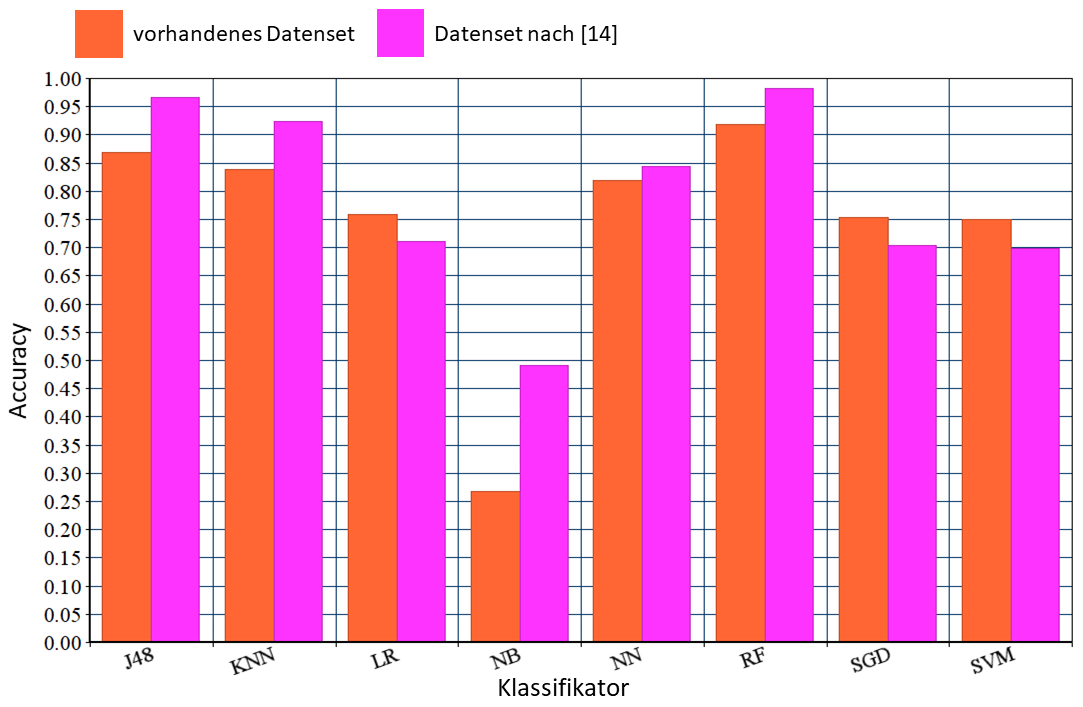
\includegraphics[width=\textwidth]{images/Klasseval}
    \caption{Übersicht der Accuracies des nicht-featurebasierten Vergleichs\label{fig:class-acc}}
\end{figure}

\subsubsection*{Weitere Evaluationsmetriken}

\begin{table}[t]
\centering
\caption{Ergebnisse der Evaluationsmetriken des nicht-featurebasierten Vergleichs}
\label{tab:class-val}
\resizebox{\linewidth}{!}{%
\begin{tabular}{|>{\hspace{0pt}}p{0.085\linewidth}>{\hspace{0pt}}p{0.147\linewidth}|>{\RaggedLeft\hspace{0pt}}p{0.16\linewidth}>{\RaggedLeft\hspace{0pt}}p{0.11\linewidth}>{\RaggedLeft\hspace{0pt}}p{0.1\linewidth}|>{\RaggedLeft\hspace{0pt}}p{0.153\linewidth}>{\RaggedLeft\hspace{0pt}}p{0.112\linewidth}>{\RaggedLeft\hspace{0pt}}p{0.102\linewidth}|} 
\cline{3-8}
\multicolumn{1}{>{\hspace{0pt}}p{0.085\linewidth}}{}           &           & \multicolumn{3}{>{\Centering\hspace{0pt}}p{0.37\linewidth}|}{\textbf{Datenset nach } } & \multicolumn{3}{>{\Centering\hspace{0pt}}p{0.367\linewidth}|}{\textbf{vorhandenes Datenset} }  \\ 
\cline{3-8}
\multicolumn{1}{>{\Centering\hspace{0pt}}p{0.085\linewidth}}{} &           & \textbf{fehlerfrei}~ & \textbf{defekt}  & \textbf{gew.}\par{}\textbf{Mittel}           & \textbf{fehlerfrei}  & \textbf{defekt}  & \textbf{gew.}\par{}\textbf{Mittel}                   \\ 
\hline
\multirow{4}{0.085\linewidth}{\hspace{0pt}J48}                 & TP-Rate   & 0,98                 & 0,93             & 0,97                                         & 0,93                 & 0,70             & 0,87                                                 \\
                                                               & FP-Rate   & 0,02                 & 0,02             & 0,07                                         & 0,30                 & 0,07             & 0,25                                                 \\
                                                               & Precision & 0,97                 & 0,96             & 0,97                                         & 0,90                 & 0,76             & 0,87                                                 \\
                                                               & F-Score   & 0,98                 & 0,95             & 0,97                                         & 0,91                 & 0,73             & 0,87                                                 \\ 
\hline
\multirow{4}{0.085\linewidth}{\hspace{0pt}KNN}                 & TP-Rate   & 0,96                 & 0,85             & 0,92                                         & 0,92                 & 0,61             & 0,84                                                 \\
                                                               & FP-Rate   & 0,16                 & 0,04             & 0,12                                         & 0,40                 & 0,08             & 0,32                                                 \\
                                                               & Precision & 0,93                 & 0,91             & 0,92                                         & 0,87                 & 0,71             & 0,83                                                 \\
                                                               & F-Score   & 0,95                 & 0,88             & 0,92                                         & 0,90                 & 0,65             & 0,83                                                 \\ 
\hline
\multirow{4}{0.085\linewidth}{\hspace{0pt}LR}                  & TP-Rate   & 0,96                 & 0,18             & 0,71                                         & 0,99                 & 0,08             & 0,76                                                 \\
                                                               & FP-Rate   & 0,83                 & 0,05             & 0,58                                         & 0,92                 & 0,02             & 0,69                                                 \\
                                                               & Precision & 0,72                 & 0,64             & 0,69                                         & 0,76                 & 0,65             & 0,74                                                 \\
                                                               & F-Score   & 0,82                 & 0,65             & 0,28                                         & 0,86                 & 0,15             & 0,68                                                 \\ 
\hline
\multirow{4}{0.085\linewidth}{\hspace{0pt}NB}                  & TP-Rate   & 0,29                 & 0,93             & 0,49                                         & 0,03                 & 0,96             & 0,27                                                 \\
                                                               & FP-Rate   & 0,07                 & 0,71             & 0,27                                         & 0,04                 & 0,97             & 0,28                                                 \\
                                                               & Precision & 0,90                 & 0,38             & 0,73                                         & 0,65                 & 0,26             & 0,55                                                 \\
                                                               & F-Score   & 0,44                 & 0,54             & 0,47                                         & 0,05                 & 0,41             & 0,14                                                 \\ 
\hline
\multirow{4}{0.085\linewidth}{\hspace{0pt}NN}                  & TP-Rate   & 1,00                 & 0,51             & 0,84                                         & 0,96                 & 0,42             & 0,82                                                 \\
                                                               & FP-Rate   & 0,49                 & 0,00             & 0,34                                         & 0,59                 & 0,04             & 0,45                                                 \\
                                                               & Precision & 0,82                 & 0,99             & 0,87                                         & 0,83                 & 0,76             & 0,81                                                 \\
                                                               & F-Score   & 0,90                 & 0,67             & 0,83                                         & 0,89                 & 0,54             & 0,80                                                 \\ 
\hline
\multirow{4}{0.085\linewidth}{\hspace{0pt}RF}                  & TP-Rate   & 0,99                 & 0,96             & 0,98                                         & 0,96                 & 0,79             & 0,92                                                 \\
                                                               & FP-Rate   & 0,04                 & 0,01             & 0,03                                         & 0,21                 & 0,04             & 0,16                                                 \\
                                                               & Precision & 0,98                 & 0,98             & 0,98                                         & 0,93                 & 0,88             & 0,92                                                 \\
                                                               & F-Score   & 0,99                 & 0,97             & 0,98                                         & 0,95                 & 0,83             & 0,92                                                 \\ 
\hline
\multirow{4}{0.085\linewidth}{\hspace{0pt}SGD}                 & TP-Rate   & 0,98                 & 0,10             & 0,70                                         & 1,00                 & 0,02             & 0,75                                                 \\
                                                               & FP-Rate   & 0,90                 & 0,02             & 0,62                                         & 0,98                 & 0,00             & 0,74                                                 \\
                                                               & Precision & 0,71                 & 0,68             & 0,70                                         & 0,75                 & 0,78             & 0,76                                                 \\
                                                               & F-Score   & 0,82                 & 0,18             & 0,62                                         & 0,86                 & 0,03             & 0,65                                                 \\ 
\hline
\multirow{4}{0.085\linewidth}{\hspace{0pt}SVM}                 & TP-Rate   & 0,92                 & 0,07             & 0,70                                         & 1,00                 & 0,00             & 0,75                                                 \\
                                                               & FP-Rate   & 0,93                 & 0,02             & 0,64                                         & 1,00                 & 0,00             & 0,75                                                 \\
                                                               & Precision & 0,70                 & 0,66             & 0,69                                         & 0,75                 & ?                & ?                                                    \\
                                                               & F-Score   & 0,82                 & 0,13             & 0,60                                         & 0,86                 & ?                & ?                                                    \\
\hline
\end{tabular}
}
\end{table}

\subsubsection*{ROC-Kurven und ROC-Bereiche}

\begin{figure}[t]
  \centering
  \subfloat[][J48 n. \cite{Moser2008}\\AUC = 0,97]{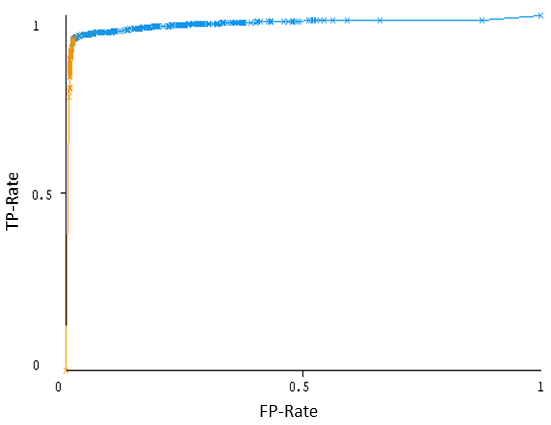
\includegraphics[width=0.25\linewidth]{images/j48_eval}} 
  \subfloat[][J48 (v. D.)\\AUC = 0,86]{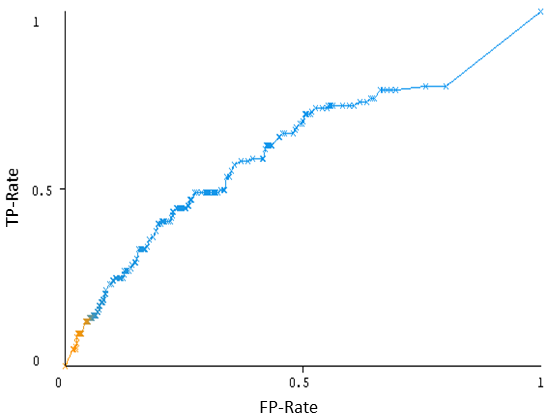
\includegraphics[width=0.25\linewidth]{images/j48_eval_feat}}
  \subfloat[][NN n. \cite{Moser2008}\\AUC = 0,89]{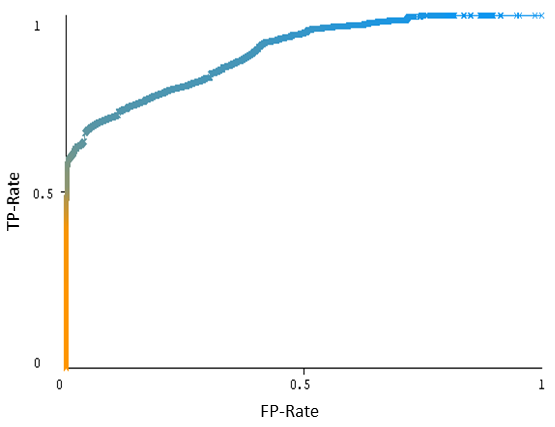
\includegraphics[width=0.25\linewidth]{images/nn_eval}}
  \subfloat[][NN (v. D.)\\AUC = 0,85]{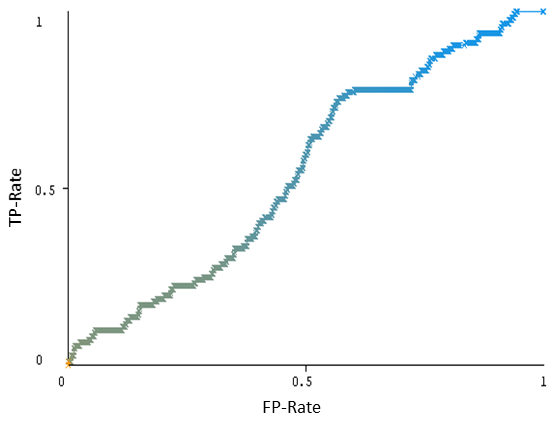
\includegraphics[width=0.25\linewidth]{images/nn_eval_feat}}
  \qquad
  \subfloat[][KNN n. \cite{Moser2008}\\AUC = 0,93]{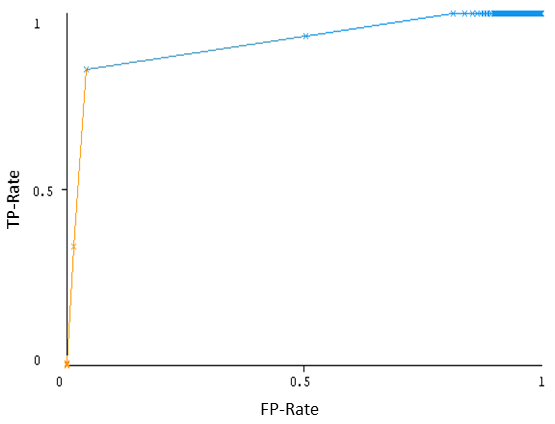
\includegraphics[width=0.25\linewidth]{images/knn_eval}}
  \subfloat[][KNN (v. D.)\\AUC = 0,77]{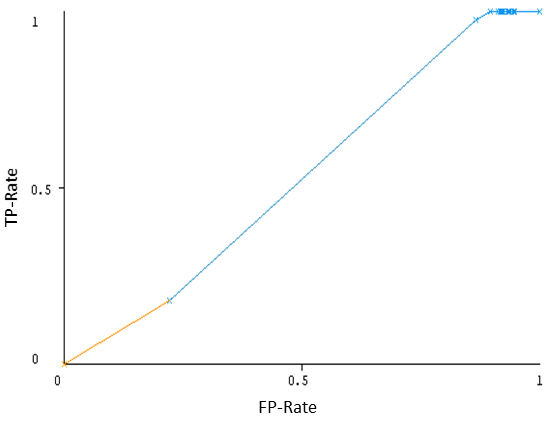
\includegraphics[width=0.25\linewidth]{images/knn_eval_feat}}
  \subfloat[][RF n. \cite{Moser2008}\\AUC = 1,00]{\includegraphics[width=0.25\linewidth]{images/rf_eval}} 
  \subfloat[][RF (v. D.)\\AUC = 0,97]{\includegraphics[width=0.25\linewidth]{images/rf_eval_feat}} 
  \qquad
  \subfloat[][LR n. \cite{Moser2008}\\AUC = 0,77]{\includegraphics[width=0.25\linewidth]{images/lr_eval}}
  \subfloat[][LR (v. D.)\\AUC = 0,73]{\includegraphics[width=0.25\linewidth]{images/lr_eval_feat}}
  \subfloat[][SGD n. \cite{Moser2008}\\AUC = 0,54]{\includegraphics[width=0.25\linewidth]{images/sgd_eval}}
  \subfloat[][SGD (v. D.)\\AUC = 0,51]{\includegraphics[width=0.25\linewidth]{images/sgd_eval_feat}}
  \qquad
  \subfloat[][NB n. \cite{Moser2008}\\AUC = 0,73]{\includegraphics[width=0.25\linewidth]{images/nb_eval}}
  \subfloat[][NB (v. D.)\\AUC = 0,61]{\includegraphics[width=0.25\linewidth]{images/nb_eval_feat}}
  \subfloat[][SVM n. \cite{Moser2008}\\AUC = 0,53]{\includegraphics[width=0.25\linewidth]{images/svm_eval}}
  \subfloat[][SVM (v. D.)\\AUC = 0,50]{\includegraphics[width=0.25\linewidth]{images/svm_eval_feat}}
  \caption{ROC-Kurven des nicht-featurebasierten Vergleichs\\(v.D. = vorhandenes Datenset)}
\end{figure}

\cleardoublepage
